\documentclass[12pt,a4paper]{ctexart}

\usepackage[final]{pdfpages}
\usepackage{fancyhdr}
\usepackage{lastpage}
\usepackage{xcolor}
\usepackage{cite}
\usepackage{graphicx}
\usepackage{pifont}
\usepackage{float}
\usepackage{amsmath}



\usepackage{url}
\usepackage{listings}
\usepackage[hidelinks]{hyperref}
\numberwithin{figure}{section}

\fancypagestyle{emptyStyle}
{
    \pagestyle{fancy}
    \fancyhf{}
}
\fancypagestyle{abstractStyle}
{
    \pagestyle{fancy}
    \fancyhf{}
    \fancyfoot[C]{\textcolor[gray]{0.6}{第\thepage 页~共\pageref{LastPage}页}}
    \renewcommand{\headrulewidth}{0pt}
    \renewcommand{\footrulewidth}{0pt}
}
\fancypagestyle{articleStyle}
{
    \pagestyle{fancy}
    \fancyhf{}
    \fancyhead[L]{\textcolor[gray]{0.6}{\leftmark}}
    \fancyhead[R]{\textcolor[gray]{0.6}{\rightmark}}
    \fancyfoot[C]{\textcolor[gray]{0.6}{第\thepage 页~共\pageref{LastPage}页}}
    \renewcommand{\headrulewidth}{0pt}
    \renewcommand{\footrulewidth}{0pt}
}
\fancypagestyle{refStyle}
{
    \pagestyle{fancy}
    \fancyhf{}
    \fancyhead[L]{\textcolor[gray]{0.6}{\leftmark}}
    \fancyfoot[C]{\textcolor[gray]{0.6}{第\thepage 页~共\pageref{LastPage}页}}
    \renewcommand{\headrulewidth}{0pt}
    \renewcommand{\footrulewidth}{0pt}
}
\setCJKmainfont{SimSun}[AutoFakeBold,AutoFakeSlant]
\setmainfont{TeX Gyre Termes}
\linespread{1.5}
\setcounter{tocdepth}{3}
\setcounter{secnumdepth}{5}
\ctexset {
section = {
name = {第,章},
number = \chinese{section},
},
subsection = {
name = {第,节},
number = \chinese{subsection},
},
subsubsection = {
name = {第,小节},
number = \chinese{subsubsection},
},
paragraph={
name = {(,)},
number = \chinese{paragraph},
runin = false,
hang = true,
},
subparagraph={
name = {,.},
number = \Roman{subparagraph},
runin = false,
hang = true,
},
}
\date{}


\title{\Huge\textbf{2023年全国大学生信息安全竞赛\\作品报告}}

\begin{document}
\definecolor{mygreen}{rgb}{0,0.6,0}
\definecolor{mygray}{rgb}{0.5,0.5,0.5}
\definecolor{mymauve}{rgb}{0.58,0,0.82}
\lstset{
    backgroundcolor=\color{lightgray},
    basicstyle = \footnotesize,
    breakatwhitespace = false,
    breaklines = true,
    captionpos = b,
    commentstyle = \color{mygreen}\bfseries,
    extendedchars = false,
    frame =shadowbox,
    framerule=0.5pt,
    keepspaces=true,
    keywordstyle=\color{blue}\bfseries, % keyword style
    language = C++,                     % the language of code
    otherkeywords={string},
    numbers=left,
    numbersep=5pt,
    numberstyle=\tiny\color{mygray},
    rulecolor=\color{black},
    showspaces=false,
    showstringspaces=false,
    showtabs=false,
    stepnumber=1,
    stringstyle=\color{mymauve},        % string literal style
    tabsize=2,
    title=\lstname
}
\pagestyle{emptyStyle}
\maketitle
\vspace{6cm}
{
    \Large\textbf{作品名称}:\textbf{\underline{\makebox[10cm]{基于TrustZone-M函数级内存地址}}}

    \textbf{\underline{\makebox[13cm]{空间随机化的可信实时系统}}}

    \textbf{电子邮箱}:\underline{\makebox[10cm]{\textbf{213211377@seu.edu.cn}}}

    \textbf{提交时间}:\underline{\makebox[10cm]{\textbf{\today}}}
}
\clearpage
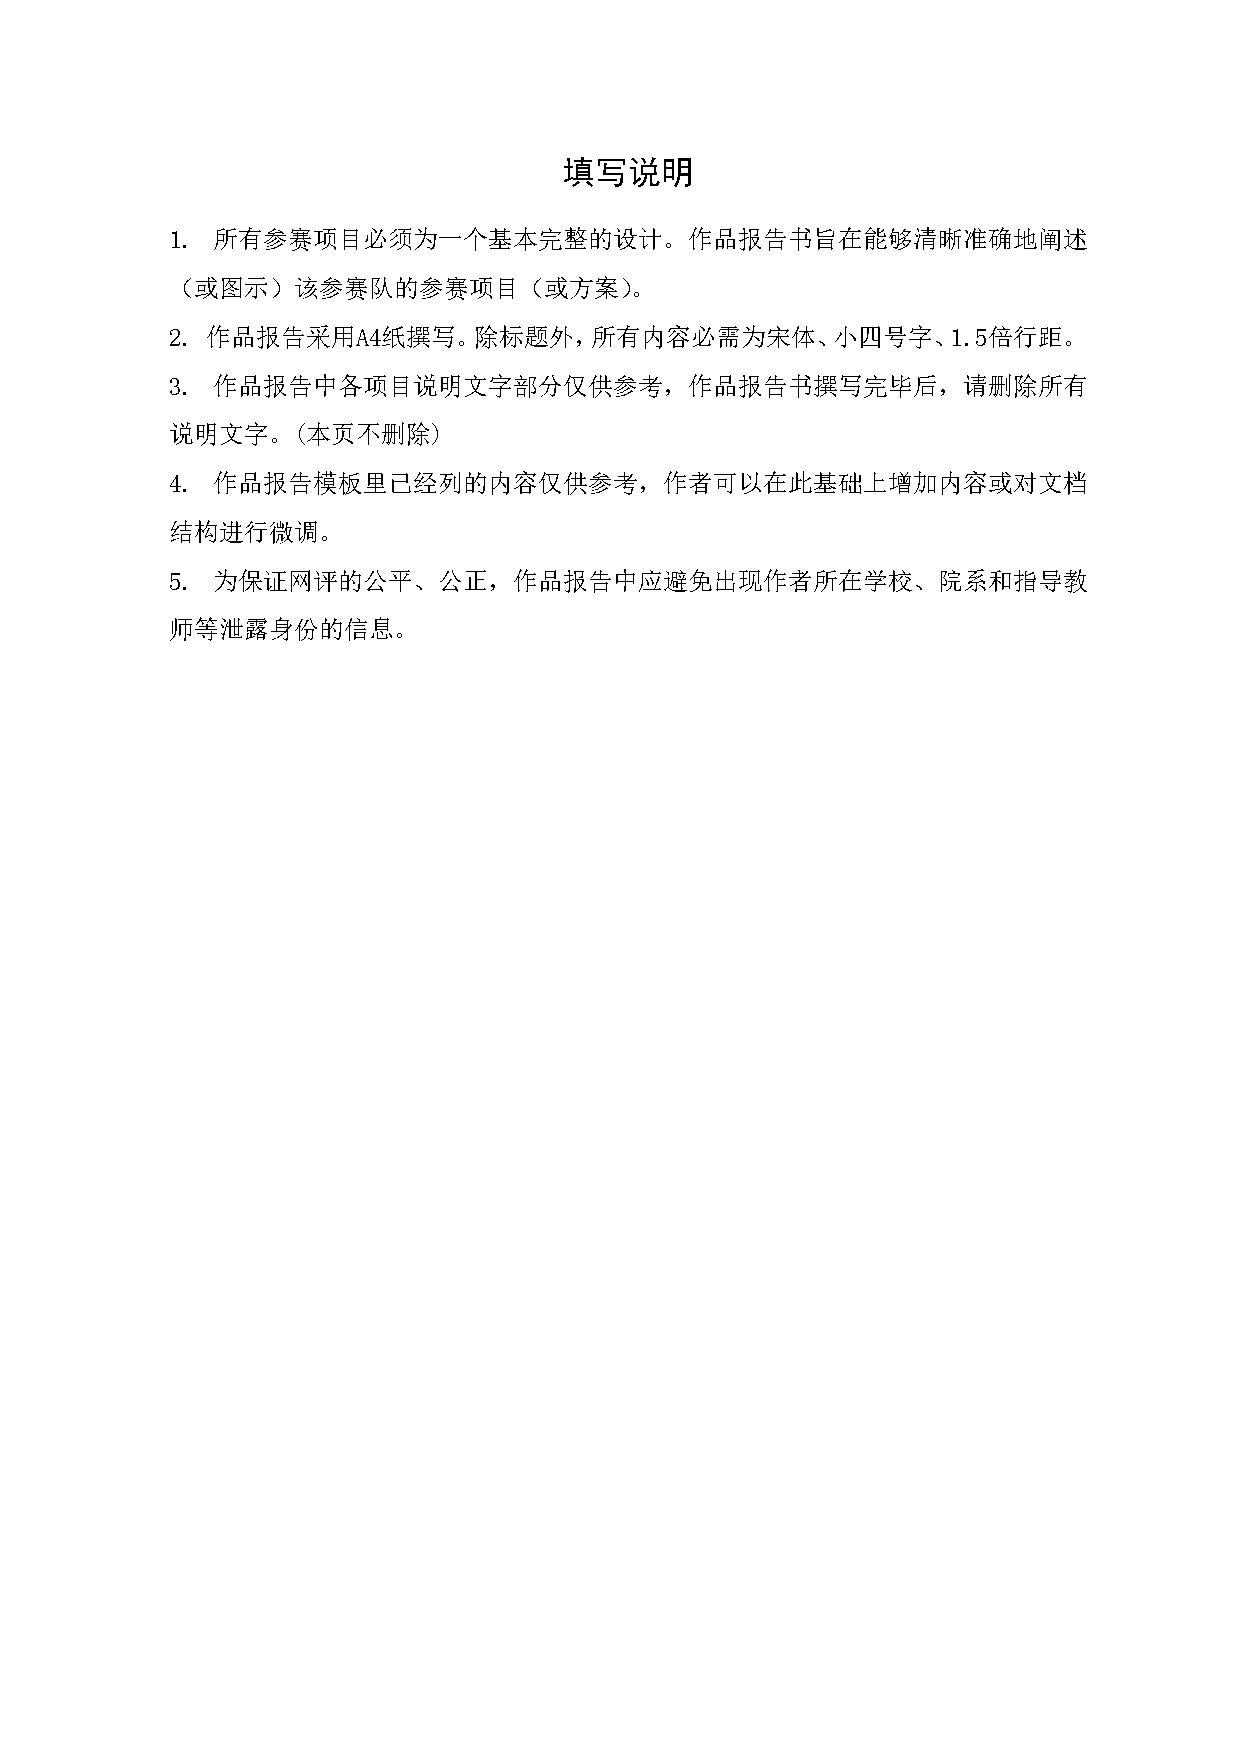
\includepdf{src/request.pdf}
\clearpage
\tableofcontents
\clearpage
\pagestyle{abstractStyle}
\setcounter{page}{1}
\section*{摘要}
\addcontentsline{toc}{section}{摘要}
简要说明创作本作品之动机、功能、特性、创新处、实用性等.
\clearpage
\pagestyle{articleStyle}
\section{作品概述}
\subsection{作品背景}
\par 近年来,伴随着信息技术的飞速发展,以智能家居、智慧交通、智慧医疗等为应用场景的物联网产业得到了迅猛发展。与此同时,物联网设备的数量也在飞速增长。到2020年底,全球物联网设备连接,如联网的汽车、智能家居设备、联网的工业设备等,数量达到了117亿,约占全球的54\%,首次超过了非物联网设备连接,如智能手机、笔记本电脑和计算机等。作为全球最大的物联网市场,中国在这一领域更是处于领先地位。到目前为止,已投入使用的物联网设备数量已经超过了144亿,预计到2025年物联网设备数量将达到270亿。
\par 虽然物联网的发展已渐成规模,但其安全问题也越来越突出。从物联网设备的角度来看,很多物联网设备是基于微控制器(Micro Controller Unit,MCU)实现的嵌入式系统,比如车载控制设备、智能锁具、无人机、可植入医疗设备等。与通用系统一样,由于嵌入式系统硬件设计不当或软件开发不当,使运行在嵌入式系统上的软件通常存在不同类型的安全漏洞,进而引发一系列的安全问题。自从2017年以来,上百个嵌入式系统的安全漏洞已经在NVD平台上被披露出来,对设备安全和用户隐私造成了严重影响。例如,谷歌Project Zero团队发现部分手机搭载的WiFi模块漏洞对用户手机造成安全威胁;家庭安防产品Ring被曝出存在可以让攻击者监控用户家庭的安全漏洞等。随着嵌入式系统安全的重要性不断提高,维护嵌入式系统的安全变得至关重要。
\par 深入研究嵌入式系统的安全威胁后发现,嵌入式系统的安全威胁很大一部分来自二进制的内存破坏攻击,主要包括代码破坏攻击(Code Corruption Attack),控制流劫持攻击(Control-flow Hijack Attack),面向数据的攻击(Data-only Attack)以及信息泄露攻击(Information Leak Attack)。其中控制流劫持攻击最为常见,例如ROP攻击等。现有针对控制流劫持攻击的防御中,主要以控制流完整性保护技术以及地址空间信息隐藏技术最具代表性。但由于嵌入式系统其低功耗、低成本的的要求,其硬件资源受到了很大的限制,导致在通用系统中的防御机制无法直接部署,尤其是基于8位,16位,32位微控制器的嵌入式系统。这些低端嵌入式系统大多处理器工作频率在100MHz以下,在存储上只有几百KB的Flash以及几十KB的RAM,并且它们普遍不支持内存管理单元(Memory Management Unit,MMU)。同时,运行在这些设备中的嵌入式系统软件一般用 C/C++语言编写实现,因此,与通用系统一样,这些嵌入式系统软件易受到内存破坏攻击,进而引发一系列的安全问题,例如攻击者可以利用内存破坏漏洞来向受攻击的应用程序中注入恶意代码,从而导致代码执行漏洞。这种攻击可能会让攻击者控制设备、窃取数据或对系统进行其他恶意行为。除此之外,还可能产生拒绝服务攻击,系统提权,数据泄露等一些列安全问题。因此,现有的内存破坏防御机制无法直接应用于低端嵌入式系统,而低端嵌入式系统尚缺乏有效的内存破坏防御机制,使其安全性受到严重威胁。
\par 一般来说,可信执行环境由可信执行环境操作系统(Trusted Execution Environment Operating System,TEE OS)以及安全服务(或称为TA,Trusted Application)构成,可信执行环境操作系统主要为用户调用安全服务提供安全的通信机制。为了满足嵌入式系统对安全日益增长的需求,ARM在2015年提出了面向Cortex-M系列芯片的TrustZone-M技术,TrustZone-M技术将嵌入式系统软硬件等资源分为安全世界和非安全世界,安全世界可以直接访问非安全世界资源,但非安全世界不能直接访 问安全资源,其对安全世界资源的访问需要通过安全世界提供的 API。这些 API 实现了身份验证,确保安全世界资源被正确使用。严格控制非安全世界与安全世界间的访问,旨在为系统提供一个TEEOS。由于其具有灵活性,易于开发,低功耗等优势,在移动终端领域,ARM公司针对Cortex-A系列芯片提出的TrustZone技术已经在大多数智能手机上得到TEEOS的配备,例如高通实现的QSEE,华为实现的TEEOS,三星实现的Knox等,该技术主要被用来提供安全支付,指纹服务,文件保密等安全服务。但是在低端嵌入式领域,目前基于TrustZone-M技术提供TEEOS的研究较少,其中较为流行的有两个,一个是ARM公司主导的开源项目Trusted Firmware-M(TF-M),另一个是Trustonic公司研发的闭源项目Knibi-M,前者虽然开源但对实时操作系统的兼容性较差,后者不开源且目前仅支持Microchip下的SAML11系列SoC(Systemon Chip),两者都可为用户提供多种安全服务,如安全加密,安全密钥管理等,但都未提供对控制流劫持攻击的安全保护机制。
\par 目前,有三个主要方向用于提高低端嵌入式系统的安全性:首先是利用低端嵌入式系统的硬件设施,例如采用前文提到的ARMv8-M 架构下的TrustZone-M 技术、系统调试单元和内存保护单元(Memory Protection Unit,MPU)等,实现内存隔离、内存检测和访问控制等安全防护措施。然而,由于嵌入式系统硬件的多样性,这要求系统开发者针对不同硬件环境实现相应的安全机制,导致可扩展性较差。此外,还需额外的硬件支持,从而增加成本和工程开销。第二个方向是利用编译器技术,在对代码进行词法和语法分析后,在重新编译现有嵌入式系统源码的过程中加入额外代码以实现特定的防御机制,从而提高系统安全性。例如,采用软件错误隔离(Software Fault Isolation,SFI)技术实现代码块隔离,利用代码多样化(Code Diversification)技术抵御代码复用攻击等。这种方法的优点是无需更改原有系统的软硬件,避免了成本和工程开发上的额外开销。但是,由于编译器在软件层面提高系统安全性,因此可能会给代码的执行效率和性能带来额外负担。最后一个方向是综合前两者,通常针对已有可信硬件的低端嵌入式系统。在编译过程中加强代码安全性,并将支持可信硬件的防御机制代码直接编译至目标代码,具有较好的可扩展性。由于此类方法本质上仍然基于编译器对代码进行重新编译,因此对系统开发具有较好的透明性。同时,得益于可信硬件的支持,对嵌入式系统的安全性以及性能也有较好的兼顾。
\par 虽然已经出现了众多的安全防护技术,如StackGuard阻止栈溢出、DEP阻止代码注入等,但是每个技术只能防御某一种特定方式的攻击,要将这些技术集成在一起实现困难且开销大,而新的攻击方式还在不断出现,为了解决这些不足,研究人员提出了从另一个角度对系统进行保护的安全技术,即地址空间布局随机化(Address Space Layout Randomization,ASLR),ASLR是一种通用计算机系统安全技术,在进程的地址空间中随机放置可执行文件、库、堆和栈的基地址位置。由ASLR执行内存地址的随机布局后,攻击者不再知道所需代码片段(例如函数或ROP gadgets)实际地址,使攻击难度大大增加。ASLR不会从系统中彻底清除漏洞,而是使攻击者利用现有漏洞更加艰巨。ASLR由PaxProject在2001年作为Linux修补程序创建,实现方法是在进程加载时,对栈基地址的4-27位共24位进行随机;对包括主程序映像、静态数据区、堆这一连续区域的基地址12-27位共16位进行随机;对共享加载库地址的12-27位共16位进行随机。ASLR技术加上数据保护执行DEP构成了一个完整的系统防护方案,DEP技术迫使攻击者使用空间中现有代码,ASLR使得这些空间中现有代码地址不可确定,由此能大大降低攻击成功的概率,在当时Linux系统中得到广泛应用。并于2007年从Vista开始集成到Windows操作系统中。之后相继出现在各种主流通用操作系统中。虽然,目前针对内存破坏攻击的运行时防御机制已广泛部署在通用系统,但这些防御机制往往需要硬件支持以减少其所引入的性能开销,比如MMU等。然而,嵌入式系统由于其低功耗、低成本的的要求,使其硬件资源受到了很大的限制,ASLR技术难以实施。
\par 因此,为保护物联网设备系统的安全,本作品针对目前控制流劫持攻击对低端嵌入式系统的威胁日益增大,缺乏有效的控制流劫持防御机制,且ASLR技术在嵌入式系统中难以实施的问题,对低端嵌入式系统的控制流劫持攻击设计实现了基于ARM TrustZone-M的函数级动态随机加载技术,该技术对整个代码空间进行随机化,包括用户程序以及实时操作系统内核,并且支持当下流行的可信执行环境操作系统Trusted Firmware,构成了整个系统原型。
\par 首先,本作品自主设计实现了基于TrustZone-M的可信执行环境操作系统,为非安全世界提供实时可信的安全服务。先为在非安全世界调用安全服务时保护安全世界间的数据通信安全,并保证其请求资源的合法性,设计安全/非安全世界的安全通信机制。同时,借助TF-M,为非安全世界提供可靠的安全服务。然后,为实现对安全服务的多任务并发调用,需要保证安全服务在非安全世界产生任务切换后依然可以恢复执行并且能将响应结果通过安全内核返回至原非安全世界任务。现有实时操作系统(如FreeRTOS)已支持任务在安全世界调用安全函数,并且可以在任务切换后恢复安全函数的执行。具体地,在切换至某一就绪任务时,非安全世界的任务调度器会检查其之前调用的安全函数是否未执行完,若存在,则会先恢复该任务所对应的安全函数并执行,然后将响应结果以函数返回的方式直接返回给该任务。这种方式虽然可以实现多任务对安全函数的并发调用,但是由于是任务直接调用安全函数,一旦安全函数存在漏洞则会破坏整个安全世界的安全性。本作品基于FreeRTOS设计了安全服务多任务并发调用技术。
\par 其次,在基于TrustZone-M可信执行环境的基础上,重点研究系统运行时低端嵌入式系统上部署地址空间布局随机化(ASLR)技术以实现对控制流劫持攻击的防御。为保证运行时系统代码地址空间布局随机化,本作品提出一种基于MPU的函数级地址空间布局随机化技术fASLR,实现系统运行时函数级的地址空间布局随机化。该技术首先设计静态信息提取技术以对系统以及函数信息进行收集与管理,实现函数运行时的实时状态感知。随后设计基于MPU的函数动态加载机制以对系统进行函数级地址空间布局动态随机化,实现对函数运行时代码地址空间布局信息的实时隐藏,最后设计函数级随机化内存管理机制,实现高利用率、高性能的函数随机加载内存管理。
\par 因此,本作品在抵抗控制流劫持攻击对低端嵌入式系统的威胁等方面具有重要的研究价值和实践意义。






\subsection{研究现状}
\par 随着ARMv8-M架构设备在物联网市场的普及,低端嵌入式系统的安全性已成为一个受到广泛关注的问题。为应对现有安全防护技术通用性较差的挑战,研究人员提出了ASLR地址空间布局随机化技术,该技术从不同的角度对系统进行保护。此外,为了提高低端嵌入式设备的安全性,现有的研究还探索了基于TrustZone-M技术的可信执行环境构建技术,该技术旨在通过安全的通信机制为用户应用程序提供可信软件服务。此外,Trusted firmware-M开源固件项目提供了一个全面的安全框架,用于保护Arm Cortex-M设备的安全性。最后,针对低端嵌入式系统面临的内存破坏攻击威胁,研究人员还致力于开发内存破坏防御技术,其中包括控制流完整性保护和地址空间信息隐藏技术。
\subsubsection{ASLR(Address Space Layout Randomization)地址空间布局随机化}
\par 自从1988年11月2日莫里斯蠕虫利用缓冲区溢出漏洞感染了上万台计算机之后,安全防护领域涌现出许多针对特定攻击方式的技术,例如StackGuard用于阻止栈溢出,DEP用于阻止代码注入等。然而,这些技术各自只能防御一种特定方式的攻击,要将它们集成在一起实现综合的防护变得困难且具有较高的实施开销。此外,攻击者不断创新,不断出现新的攻击方式,这使得传统的防护技术面临挑战。
\par 为了解决这些不足,研究人员开始探索一种从另一个角度对系统进行保护的安全技术,即地址空间布局随机化(ASLR)。ASLR的核心思想是通过随机化系统的内存布局,使得攻击者无法预测和利用特定的内存地址,从而增加攻击的难度。它引入了一定程度的不确定性和随机性,使得攻击者难以准确定位和利用系统中的关键函数或数据。
\par 具体而言,ASLR通过在系统启动时对代码、堆、栈和库等内存区域的基址进行随机化,使得它们在每次运行时都位于不同的内存位置。这种随机化使得攻击者无法事先获知这些内存区域的准确位置,从而破坏了攻击者依赖特定地址的攻击方式,如代码注入和ROP(Return-Oriented Programming)攻击。
\par ASLR的实现依赖于操作系统的支持,它需要对内核和应用程序进行修改和扩展。通常,操作系统会提供一种机制来生成随机的内存布局,并在运行时将这些随机值应用于相应的内存区域。此外,ASLR还可以结合其他防护技术,如栈随机化和堆随机化,以提供更强大的保护效果。
\par ASLR最早由Pax项目在2001年作为Linux修补程序创建。其实现方法包括对进程加载时的不同内存区域进行随机化,以使攻击者难以准确定位和利用特定的内存地址。
\par 具体来说,在ASLR的实施中,栈基地址的4-27位共24位会被随机化,而主程序映像、静态数据区和堆这一连续区域的基地址的12-27位共16位以及共享加载库地址的12-27位共16位也会被随机化。通过这种方式,ASLR增加了系统内存布局的不确定性,使得攻击者无法事先获知关键代码和数据的准确位置。
\par 在与数据保护执行(Data Execution Prevention,DEP)结合使用时,ASLR构成了一个完整的系统防护方案。DEP技术迫使攻击者只能使用空间中已有的代码,而ASLR使得这些代码的地址变得不可预测。这样的组合极大地降低了攻击成功的概率,在当时的Linux系统中得到广泛应用。从Windows Vista开始,ASLR也被集成到Windows操作系统中,并随后出现在各种主流通用操作系统中。
\par 然而,在嵌入式系统中实现ASLR技术面临一些困难。首先,嵌入式系统通常具有有限的地址空间,这限制了ASLR的可行性。由于地址空间较小,随机化内存布局可能导致碎片化和资源浪费,对系统的性能和效率产生负面影响。其次,嵌入式系统缺乏像操作系统加载器这样的硬件支持,这使得实施ASLR技术变得更加困难。ASLR依赖于操作系统对内存区域进行随机化,然而在嵌入式系统中,没有通用的加载器来执行这些操作。此外,嵌入式系统通常具有有限的资源,如处理能力和存储容量,这进一步限制了实现ASLR的可能性。因此,针对嵌入式系统的ASLR技术需要考虑到这些限制,并采用特定的优化策略和算法,以在有限的资源和硬件条件下提供有效的内存随机化保护。为解决这些问题,本文提出了以函数为粒度的函数动态随机加载技术,并建立相应的安全执行环境。通过这种方法,嵌入式系统能够在受限的资源和硬件条件下,实现对函数地址的随机化,从而提高系统的安全性。

\subsubsection{基于TrustZonc-M技术的可信执行环境构建技术}
一般来说,可信执行环境由可信执行环境操作系统(Trusted Execution EnvironmentOperating System,TEE OS)以及安全服务(或称为TA,Trusted Application)构成,可信执行环境操作系统主要为用户调用安全服务提供安全的通信机制。ARM TrustZone技术是ARM 公司2008年提出的处理器级系统范围的可信执行环境解决方案,为Cortex-A 系列芯片提供安全的可信执行环境支持。目前,大多数智能手机已配备有TrustZone的芯片以及可信执行环境操作系统,并安装了相应的安全服务以用于手机的安全支付、指纹服务、文件保密等。为了满足低端嵌入式系统对安全日益增长的需求,ARM在2015年提出了面向Cortex-M系列芯片的TrustZone-M\cite{armv8mARM}技术并支持ARMv8-M架构设备。基于TrustZone-M的低端嵌入式系统在物联网市场正逐渐普及,然而,面向资源受限设备的可信执行环境研究在学术界和工业界尚处于起步阶段。

\paragraph{TrustZone-M 技术的安全机制}
\par TrustZone-M面向资源受限的低端嵌入式设备,利用系统级的硬件隔离技术将系统资源分为安全/非安全世界。安全世界的资源可以访问非安全世界的资源,反之则会产生错误。下面从编程模型、资源分配以及异常处理三方面对TrustZone-M进行介绍。
\par \textbf{编程模型:}自ARMv7-M架构开始,处理器有两种操作模式:thread模式和 handler模式。在thread模式下,处理器用于执行应用程序代码且其访问权限级别可以处于特权态(Privileged)或者非特权态(Unprivileged)。在 handler模式下,处理器用于执行异常处理程序代码且总是特权态。ARMv8-M架构引入TrustZone-M技术后,处理器额外增加了两个安全状态:安全态(Secure State)和非安全态(Non-secure State),这两个状态和处理器操作模式互相独立,即每个安全状态都有thread或者handler两个操作模式。安全状态不是由某一安全位控制,而是取决于处理器所访问的内存地址或者IO地址是映射在安全还是非安全世界。若该内存映射在安全世界,则处理器状态为安全态,反之,则为非安全态。不同的安全状态以及处理器操作模式对应不同的栈指针寄存器,共有 PSP\_NS、PSP\_S、MSP\_NS、MSP\_S 四个栈指针寄存器,程序当前所使用的寄存器由当前处理器的状态决定,其中,thread 模式可以使用PSP(Process Stack Pointer)栈指针寄存器,也可以使用MSP(Main Stack Pointer)栈指针寄存器,而handler模式只能使用MSP栈指针寄存器。此外,支持 TrustZone-M 的ARMv8-M架构为两个安全状态分配了独立的CONTROL寄存器以及异常处理控制寄存器(PRIMASK、FAULTMASK、BASEPRI)。
\par \textbf{安全/非安全世界的切换通过三条新引入的指令实现:}用于从非安全世界跳转至安全世界指令BXNS(Branch and Exchange Non-secure)、安全网关指令SG(Secure Gateway)以及用于从安全世界链接跳转至非安全世界指令BLXNS(Branch with Link and Exchange Non-secure)。安全世界程序调用非安全世界程序一般使用BLXNS指令,然而,非安全世界程序不能直接调用安全世界程序,它必须首先跳转至该程序在一块特殊的安全世界内存区域的入口,该内存区域被称为非安全可调用(Non-Secure Callable,NSC)区域。为保证入口是从非安全世界至安全世界的有效跳转,入口的第一条指令必须为SG。当安全世界程序执行完成后,使用BXNS指令即可返回至非安全世界。此外,异常处理时也可以发生安全状态的切换。
\par 基于TrustZone-M设备的系统运行机制如下图\ref{fig:TrustZone-M1}所示,当设备上电启动之后,首先会执行安全世界的固件程序,包括安全启动(\textcircled{1})以及TrustZone-M的初始化(\textcircled{2}),其中,TrustZone-M的初始化主要涉及对资源的安全属性划分与配置。然后,由安全世界将控制权转交给非安全世界的启动代码(\textcircled{3})并进行非安全世界的初始化(\textcircled{4}和\textcircled{5})。在此之后,系统运行非安全世界的应用程序,在运行过程中,非安全世界可以通过调用安全世界的API以在安全世界执行相应任务,同样的,安全世界在执行过程中也可以通过回调函数调用非安全世界的函数(\textcircled{6})。
\begin{figure}[h]
    \centering
    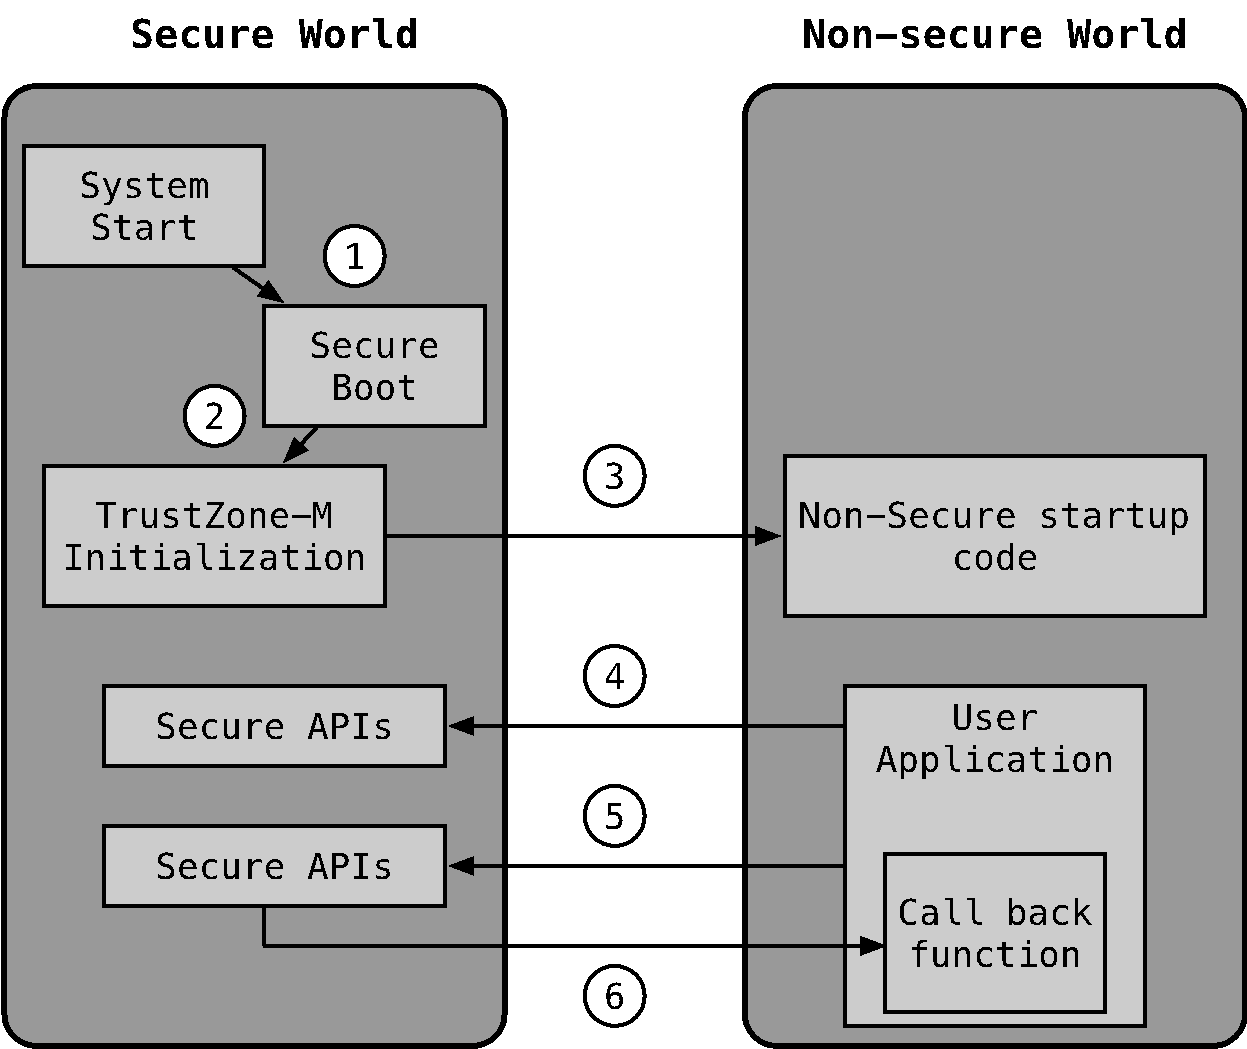
\includegraphics[scale=0.5]{graph/2.png}
    \caption{基于TrustZone-M的系统运行机制}
    \label{fig:TrustZone-M1}
\end{figure}
\par \textbf{资源分配:}TrustZone-M技术为ARMv8-M架构设备提供基于硬件的内存隔离机制,处理器根据内存映射可以对所有资源(包括内存,外设等)进行访问,其内存资源可以设置不同的安全属性以及资源访问控制权限。内存资源可以通过安全属性单元(Security Attribution Unit,SAU)进行安全区域的划分,区域数量由芯片制造商决定,一般为8个区域,SAU只能在处理器处于安全状态下被配置。除SAU之外,安全属性还可以通过实现定义属性单元(Implementation Defined Attribution Unit,IDAU)来进行配置。对某一内存区域来说,其安全属性取决于SAU和IDAU对其配置的共同作用结果,通过对两种配置取逻辑或操作以确定最终的安全属性。此外,内存资源可以通过内存保护单元(Memory Protection Unit,MPU)进行内存访问权限的设置,包括读权限、写权限、可执行权限。任何未遵守该权限要求的访问将会触发HardFault异常处理,安全/非安全世界各有一个MPU。

\par \textbf{异常处理:}在支持TrustZone-M的设备上,通过嵌套向量控制器(Nested Vector Interrupt Control,NVIC)可以设置异常处理为安全或者非安全属性。ARM的M系列处理器在异常处理时支持硬件级的异常上下文保存与恢复。TrustZone-M的异常处理操作模式切换如图\ref{fig: Exception handling operation mode switch}所示,一旦异常被触发,处理器根据向量表(Vector Table)决定异常处理程序并进行控制流跳转,其操作模式自动切换成handler模式并且使用MSP作为异常处理时的栈指针,而异常触发前的上下文信息会自动的压入在先前执行的栈中,称为异常栈帧(Exception Frame)。在ARMv8-M Baseline架构下的异常栈帧的结构如图\ref{fig:Exception frame stack structure}所示\cite{armv8mEaih},包括状态寄存器xPSR、异常返回地址、链接寄存器LR以及通用寄存器R0-R3的值。同时,当前链接寄存器LR将会载入一个称为EXE\_RETURN的特殊值,该特殊值记录着异常返回时处理器的状态信息,如处理器的操作模式、安全状态、使用的栈寄存器等。当异常返回(即跳转至EXE\_RETURN)时,异常栈帧中的内容会自动的载入其对应的寄存器中以恢复异常触发前的上下文,控制流也回到异常触发前的位置继续执行。

\paragraph{基于TrustZone-M的可信执行环境研究应用}
\par 迄今为止,已有相关公司以及研究团队利用TrustZone-M技术提出面向资源受限设备的可信执行环境。Trusted Firmware-M(TF-M)是ARM公司针对ARMv8-M架构(包括Cortex-M23,Cortex-M33,Cortex-M55处理器)或者双核平台提供的一个基于双世界架构(即安全世界和非安全世界)的可信执行环境。它符合ARM公司为物联网嵌入式系统提出的首个行业安全平台架构PSA(Platform Security Architecture)标准,并由ARM公司主导开源。TF-M在ARMv8-M架构上利用TrustZone-M的隔离机制将程序执行环境划分为非安全处理环境(Non-secure Processing Environment,NSPE)以及安全处理环境(Secure Processing Environment,SPE)。在安全处理环境中,TF-M为用户层提供多种安全服务,比如安全启动、安全密钥、安全存储等。其内核层利用SAU以及MPU对安全服务之间进行运行时隔离,并为安全服务之间以及NSPE与安全服务之间提供了安全的通信、安全中断处理等机制,NSPE中的程序可以通过TF-M提供的PSA功能API对安全服务进行调用。然而,用户程序对安全服务进行调用时会进入阻塞直到调用结果返回,这是因为TF-M为满足PSA提出的高等级隔离,TF-M中安全服务的调用模型为信号驱动型且由TF-M内核提供进程间通信(Inter-processing Communication,IPC)机制负责与安全服务进行交互。
\begin{figure}[htbp]
    \centering
    \begin{minipage}[t]{0.4\textwidth} %textwidth值小于0.25,或者linewidth小于0.5,不过这里设置textwidth比设置linewidth效果好一些
        \centering
        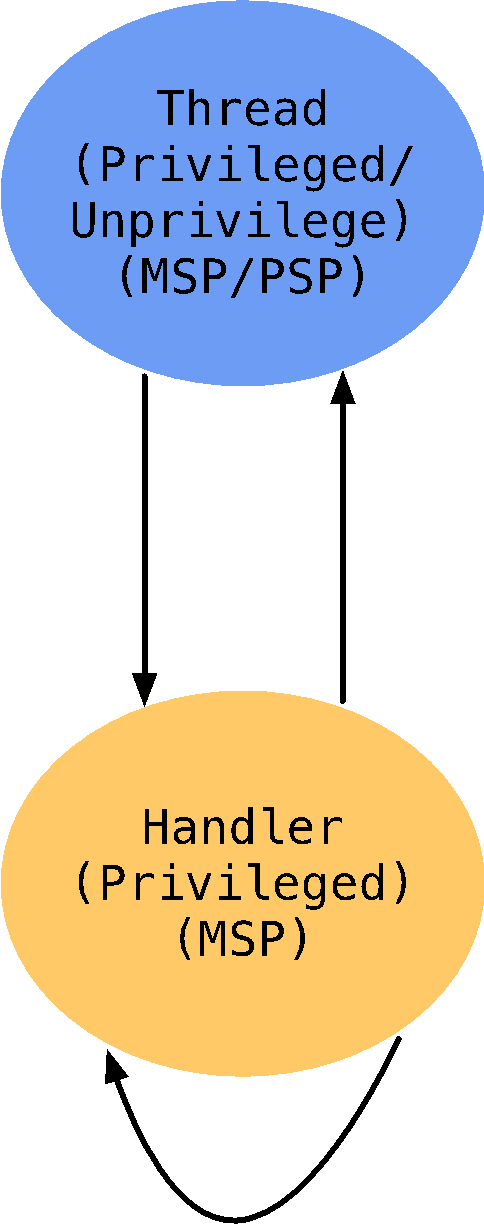
\includegraphics[scale=0.25]{graph/3.png}
        \caption{异常处理操作模式切换}
        \label{fig: Exception handling operation mode switch}
    \end{minipage}
    \hspace{0.58in} % 两图片之间的距离
    \begin{minipage}[t]{0.4\textwidth}%textwidth值小于0.25
        \centering
        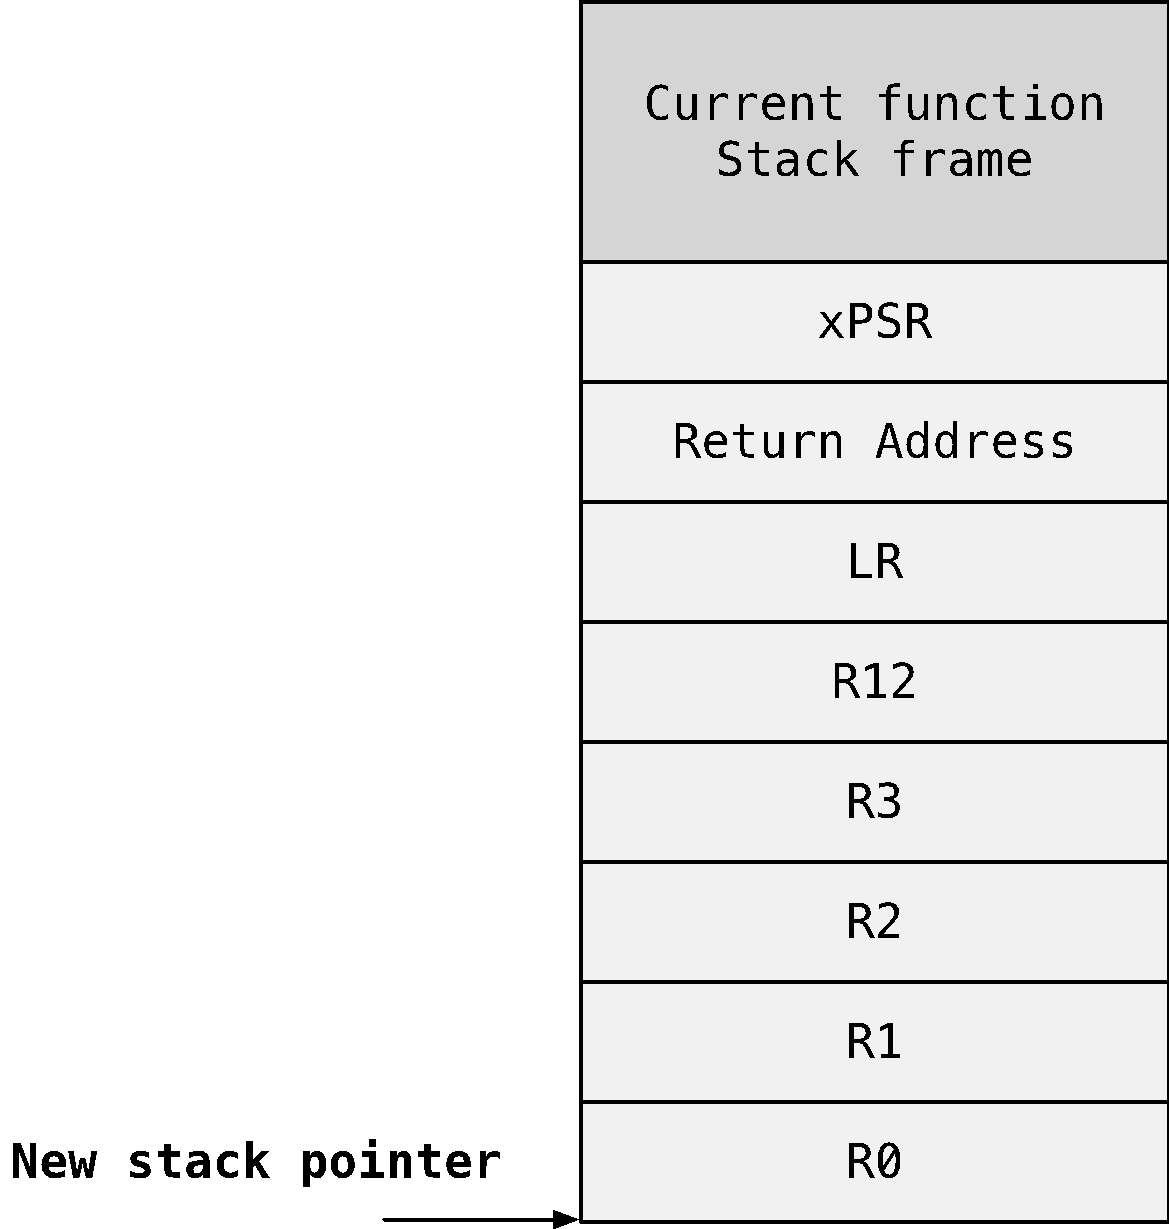
\includegraphics[scale=0.25]{graph/4.png}
        \caption{异常帧栈结构}
        \label{fig:Exception frame stack structure}
    \end{minipage}
\end{figure}
\par Trustonic公司与Microchip公司联手推出了基于TrustZone-M的Knibi-M双世界架构可信执行环境,它针对裸机版本的SAML11\cite{Microchip}设计开发,用于为该设备提供可信的安全服务。它包括内建的密码算法和安全数据存储,可以被集成到支持TrustZone-M的不同微处理器上。Knibi-M利用TrustZone-M以及安全网关(Secure Gateway)\cite{ARMv8-MATO}以与传统的非安全世界应用进行隔离。安全世界包括Knibi-M引导(Bootloader)以及多个安全服务的操作系统,可以为非安全世界中的应用程序提供安全的功能。非安全世界包括主要的应用程序以及调用安全服务的接口。Knibi-M含有一个设备唯一的密钥(目前仅支持SAML11 KPH版本),它是设备出厂时由制造商安装的,它可以为Knibi-M提供消息证明,证明的消息可以被Trustonic的云服务商认证,从而证明该消息来自一个已知的设备。目前,Knibi-M只支持裸机版本SAML11,并不支持其他型号的ARMv8-M设备且未支持实时操作系统。
\par Oliveira\cite{uTango}等人利用TrustZone-M技术,针对ARMv8-M设备提出了基于多世界(Multi-world)架构的可信执行环境操作系统UTANGO。它根据最小权限原则,利用TrustZone-M的安全状态控制器(即SAU或IDAU)降低安全服务的执行权限并使其在非安全世界下执行,并为非安全世界的程序以及各个安全服务提供互相隔离且相同的运行环境,该运行环境称为非安全虚拟世界(Non-secure Virtual World,NSVW)。为了能切换不同的NSVW,每个NSVW都有一个世界控制块(World Control Block,WCB)用于记录其上下文内容,系统运行时UTANGO在安全世界为非安全世界运行的所有NSVW进行调度并为各个NSVW之间提供数据通信接口。然而,由于在世界切换过程中涉及大量的上下文内容保存与恢复,为系统带来较严重的性能开销。另外,目前UTANGO暂不支持抢占式世界切换,非当前NSVW产生的异常难以得到及时的处理,对系统实时性有一定影响。
\par 现有TrustZone-M的可信执行环境的相关工作,其功能主要是为安全服务提供可信的执行环境并为用户提供基于不同安全通信机制的安全服务调用。然而,目前开源可信执行环境中的安全通信机制交互过程复杂,相对于资源和性能受限的低端嵌入式系统来说具有较大代码和性能开销,且可扩展性较差,例如TF-M的信号驱动型安全服务以及IPC的通信机制、UTANGO中NSVW之间繁重的上下文切换等。除此之外,现有基于双世界架构的安全通信机制只允许执行单个安全服务,并未考虑实时操作系统环境下多任务对安全服务进行并发调用需求,导致多任务下对安全服务的调用易受到阻塞,对多任务间的实时协同性产生影响。然而,TF-M以及Knibi-M的安全通信中对安全服务请求过程的参数检查,隔离机制等为本论文设计安全通信机制提供了一种可行思路。另外,本论文针对现有可信操作系统未支持多任务场景下安全服务的并发调用问题,基于现有实时操作系统FreeRTOS,设计多任务场景下对安全服务的并发调用技术。

\subsubsection{ Trusted firmware-M架构设计}
\par Trusted Firmware-M(TF-M)是由Arm开发的开源固件项目,旨在为物联网(loT)设备提供安全的运行环境。TF-M旨在提供一个可配置和可裁剪的安全固件平台,以支持从小型嵌入式设备到高端安全系统的多种应用场景。TF-M的架构是模块化的,允许使用者在不影响其他模块的情况下添加或删除安全服务。
\paragraph{Trusted firmware-M架构及安全机制}
\par TF-M 采用了两个核心概念:Secure Processing Environment(SPE)和Non-Secure Processing Environment(NSPE)。SPE 是一个安全执行环境,可以保护关键数据和代码免受未经授权的访问和修改。NSPE 是一个普通的执行环境,可以访问所有的硬件资源。TF-M 提供了一组安全服务,例如安全启动、加密解密、密钥管理、认证和授权等,这些服务可以在SPE中运行,以保证安全性。
\par TF-M的系统整体架构设计如图所示。整个TF-M部署在安全世界(SPE)中,为安全/非安全世界提供安全服务,主要由安全启动(Secure Boot)、TF-M内核(TF-M Core)以及安全服务(Secure Service)组成。
\begin{figure}[h]
    \centering
    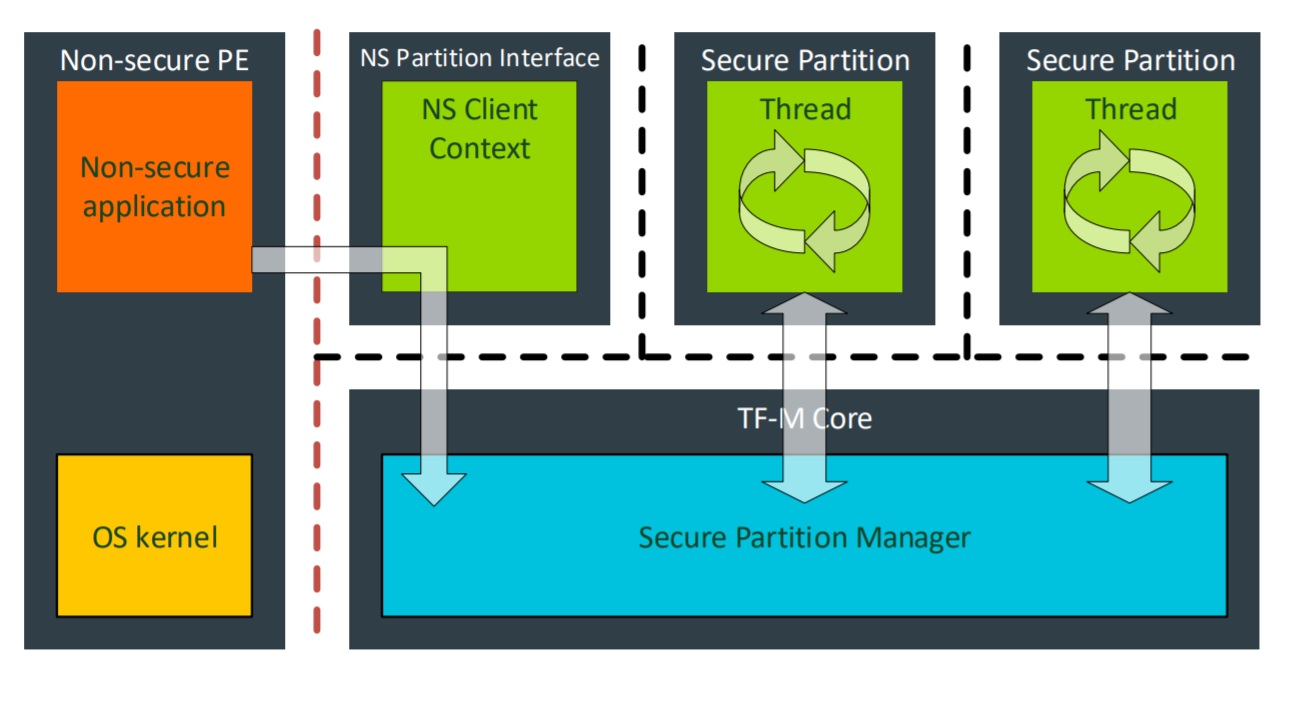
\includegraphics[scale=0.5]{graph/1.jpg}
    \caption{Trusted Firmware-M架构}
\end{figure}
\par 在Trusted Firmware-M的背景下,安全启动负责在固件映像被加载和执行之前验证其真实性和完整性。它通过根据设备安全引导固件中存储的一组受信任的密钥检查固件映像的数字签名来执行此验证。安全启动可以对SPE (Secure Processing Environment)和 NSPE (Non-Secure Processing Environment)固件映像进行身份验证。NSPE映像在设备的非安全世界中执行,而SPE映像在安全世界中执行。如果固件映像未通过Secure Boot验证,则会被拒绝,设备将无法执行它。这可以防止攻击者在设备上执行未经授权的代码,从而保护设备及其数据免受恶意活动的侵害。
\par TF-M内核是TF-M的主要组成部分之一,它是一个基于微内核的安全操作系统内核。TF-M core的主要功能是提供安全隔离、通信控制和安全执行,主要模块包括IPC、SPM、Interrupt Handling。其中,IPC 用于在SPE和 NSPE之间进行通信。它提供了一种安全的方式,以便在受保护的环境内传递数据和控制信息。SPM用于管理和控制在SPE中运行的各个安全分区。SPM使得多个安全分区可以在同一硬件平台上运行,并且可以互相隔离。Interrupt Handling用于管理和处理来自设备的中断请求。TF-M内核通过在SPE和NSPE之间传递中断请求,确保了所有中断的安全处理。TF-M内核还包括一些其他的辅助模块,比如Secure Entry/Exit和Secure Attribution等,用于在SPE和NSPE之间进行安全的上下文切换和资源分配。
\par 安全服务负责向安全/非安全世界提供具有较高安全需求的功能实现并由安全内核负责对其进行调用,如安全储存、安全启动、加密等。每一个安全服务具有唯一标识符SID(Service ID)且有统一的函数调用入口。为统一调用接口,每个安全服务都可以通过SID和version两个参数被非安全世界用户进行调用,其中,SID参数是要调用的安全服务的唯一标识符,version是请求的信任根服务版本。NSPE的用户通过PSA API发送请求后,由SPM将请求打包成消息并转发到相应服务处理程序的函数。
\par 非安全世界在调用安全世界的安全服务时,其整个通信过程如下图所示,可以分为三个阶段:(1)请求阶段:非安全世界任务发起安全服务的请求至特定的API并最终交给TF-M内核;(2)执行阶段:TF-M内核验证客户端的身份和权限,然后根据请求中指定的安全服务标识符,将请求转发给对应的安全服务并等待其响应结果;(3)响应阶段:安全服务执行结束并返回执行结果给 TF-M内核,TF-M内核收到安全服务的执行结果后,会根据请求的类型和参数,将结果通过特定API返回给客户端。

\paragraph{TF-M应用研究}
\par 2016年,P. Wägemann等人\cite{trustzone-firmware}设计和实现一种基于TrustZone的安全固件架构,利用TF-M作为基础来保护物联网设备免受各种攻击。该安全固件架构基于TrustZone技术,该技术提供了硬件级别的安全隔离。研究者利用TrustZone的两个不同的执行环境,即"安全世界"和"非安全世界",来实现安全隔离。安全世界运行在受保护的安全模式下,而非安全世界则运行在常规的非安全模式下。通过使用TrustZone和TF-M,研究者实现了更强大的安全隔离。安全世界被限制为只能通过安全接口与非安全世界进行通信,这确保了安全世界的代码和数据无法被非安全世界访问或篡改。安全世界中的关键功能和数据被保护在一个安全的容器中,只有经过授权的访问才能获取。为了保护设备中的关键数据和执行,研究者采取了多种安全措施。首先,通过在安全世界中运行关键功能,确保只有经过授权的代码可以访问和执行这些功能。其次,使用加密算法对关键数据进行加密,以防止未经授权的访问。此外,安全世界中的代码和数据也可以受到完整性检查的保护,以确保其未被篡改。但这项研究可能存在一些实施上的挑战。例如,由于物联网设备的资源限制,安全固件的实现可能会受到性能和存储限制的影响。此外,研究中可能没有对所有可能的攻击进行全面考虑,导致可能存在其他安全漏洞。
\par S.Kumar等人进行的研究\cite{secure-firmware-updates}旨在解决物联网设备固件更新过程中的安全性问题。研究者提出了一种安全的固件更新机制,利用ARM TrustZone和TF-M来确保固件的完整性和机密性。他们采用了多种机制来防止恶意固件的注入。首先,实现了固件验证机制,通过数字签名或哈希算法对固件进行验证,确保固件的完整性。只有通过验证的固件才能被接受和安全地更新。其次,实现身份认证机制用于验证固件的来源和合法性,以防止非法固件的注入。这可以通过使用公钥基础设施(Public Key Infrastructure)或其他身份验证机制来实现,确保请求只有来自信任的源头才能被接受。通过使用ARM TrustZone和TF-M,研究者确保了固件更新过程的安全性。安全世界中的代码负责处理固件更新的操作,并通过安全接口与非安全世界进行通信。固件在安全世界进行验证和认证后,才能被接受并安全地更新到设备中。这样可以防止未经授权的固件更新,同时确保更新的固件是合法和可信的。但本研究实现的安全固件更新机制在实现过程中无法确保在固件更新过程中,包括固件的验证、加载和替换过程的所有环节都是安全的。
\par  Arm Limited 公司\cite{trusted-firmware}基于前人的研究,为物联网设备提供一个全面的安全框架,提供了全面的安全功能应用,以应对不断增长的安全威胁。Arm Limited 的研究方案主要集中在设计和实现 TF-M 的安全特性和功能。这些功能包括安全引导(Secure Boot)、安全分区(Secure Partitioning)和安全通信(Secure Communication)等。相较于以往的研究,Arm Limited 在 TF-M 的研究中取得了一些突破。他们提供的全面安全框架集成了安全引导、安全分区和安全通信等关键功能,使得物联网设备能够综合地应对安全挑战。其次,他们基于 Arm Cortex-M 架构,充分利用硬件安全特性和 TrustZone 技术,提供了更强大的安全隔离和保护机制。但是,尽管 Arm Limited 的研究提供了一个全面的安全框架,但也存在一些限制和挑战。例如,由于物联网设备的多样性和复杂性,将该安全框架应用于不同设备可能需要定制化的适配和配置,这将增加了开发和部署的复杂性。此外,该研究可能没有充分考虑到未来可能出现的新型安全威胁和攻击方式。
\par J. Kim等人的研究\cite{secure-bootloader}旨在设计一种基于 TF-M 的安全引导程序,以提供物联网设备的安全引导功能。研究者设计了一个基于 TF-M 的引导程序,该程序能够确保设备在启动过程中的安全性,并保护设备免受恶意固件的加载和执行。研究者利用 TF-M 提供的安全特性,如安全分区和安全存储,来实现安全引导过程。安全隔离使引导程序运行在安全分区中,与非安全分区进行隔离。这样可以防止恶意固件或非授权代码对系统的攻击和篡改。只有通过授权的引导程序可以加载和执行,确保引导过程的完整性和可信性。安全验证使引导程序和关键数据存储在安全存储中,并通过安全存储的保护机制进行访问控制。在引导过程中,TF-M可以验证引导程序的完整性和真实性,确保只有经过验证的固件被加载和执行。然而,这项研究还存在一些潜在的缺陷和不足,比如如何确保引导程序的完整性和可信性,以及应对物理攻击和侧信道攻击的挑战。此外,实施安全引导可能需要额外的硬件支持或安全认证机制,将增加设备的成本和复杂性。

\subsubsection{面向低端嵌入式系统的内存破坏防御技术}
\par 内存破坏问题一直是计算机安全领域研究的重点之一,它一般存在于C或者C++编写的软件中,内存破坏攻击都是通过触发一个内存错误以实现攻击,比如悬挂指针,数组越界访问等。根据Szekeres\cite{6547101}等人对内存破坏攻击的调研,攻击者可以利用内存破坏漏洞实现代码破坏攻击(Code Corruption Attack),控制流劫持攻击(Control-flow Hijack Attack),面向数据的攻击(Data-only Attack)以及信息泄露攻击(Information Leak Attack)。其中,尽管在低端嵌入式系统安全领域已存在些许安全机制以抵御不同类型的内存破坏攻击\cite{7958583,8806725,almakhdhub2020mu},然而,控制流劫持攻击依旧是该领域的主要威胁,现有针对控制流劫持攻击的防御中,主要以控制流完整性保护技术以及地址空间信息隐藏技术最具代表性。
\paragraph{控制流完整性保护技术}
\par 控制流完整性保护技术是指对控制流转移进行检查以防御控制流劫持攻击。控制流劫持攻击是由于内存安全问题所引起的针对间接控制流转移的篡改,目前可分为前向控制流转移攻击和后向控制流转移攻击。前向是指攻击者通过篡改函数指针或者虚函数表等来达到转移控制流的目的,而后向则是指通过篡改函数返回地址来改变控制流转移,因此控制流完整性保护可分为前向控制流完整性保护以及后向控制流完整性保护。由于前向控制流完整性保护性能很大一部分取决于CFI的目标集(即CFI所保护的间接跳转的集合)中产生调用的次数,而对于低端嵌入式系统来说,其代码量较少\cite{almakhdhub2020mu}导致其CFI目标集也相对较少,因此可以通过直接部署通用系统的前向完整性保护技术\cite{burow2017control}以保证前向控制流完整性。然而,对于基于返回地址的后向完整性保护来说,函数的返回地址由于其在程序中所占数量庞大,且更容易被攻击者所利用\cite{almakhdhub2020mu},因此后向完整性保护在低端嵌入式系统领域依然具有较大的挑战性。
\par Sun等人\cite{9152803}针对嵌入式系统提出了操作完整性(Operation Execution Integrity,OEI),并设计了一个端到端的系统OAT(OEI ATtester),该系统可在基于ARM的嵌入式设备上实现OEI的远程认证。OEI包括控制流完整性以及数据流完整性。在控制流完整性上,OAT利用远程证明机制来提高在嵌入式设备上的性能,它结合对控制流转移以及返回的跟踪,计算其相对应的哈希值并发送给远程验证服务器,保证对控制流完整性前向和后向的双覆盖,使远程验证者能够快速地重构控制流并对其完整性进行验证。然而,该防御机制需要额外硬件支持(比如可信执行环境,额外的处理器核心等)并且仅能够检测攻击但不能终止攻击。在针对后向控制流完整性保护的研究中,影子栈\cite{8835389}被证明可以提供对返回地址的完整性保护,因此受到广泛关注。CFI-CaRE\cite{nyman2017cfi}利用TrustZone-M技术将影子栈进行强制硬件隔离从而实现后向完整性保护,每次对影子栈的操作需要面临一次系统调用以及一次安全/非安全世界的切换。RECFISH\cite{walls2019control}结合CFI技术以及影子栈并通过插桩技术直接应用到嵌入式系统的二进制文件上,从而不需要源码的支持,但是由于它将影子栈部署在特权区域(Privileged Region),所以每次函数返回时必须经过一次系统调用。因此,这两种方法都面临较大的性能开销。随后,Silhouette\cite{zhou2020silhouette}利用平行影子栈(Parallel Shadow stack)\cite{dang2015performance}技术镜像一个相同大小的栈,使用MPU对影子栈以及用户代码区域进行权限划分,最后利用基于ARMv7-M指令集的存储硬化(Store Hardening)技术对用户代码区域进行权限转换,从而保证影子栈与用户代码的地址空间隔离。但受限于ARMv7-M指令集,部分指令的转换(例如浮点存储指令)会带来较大的空间和时间开销。除了利用影子栈实现控制流完整性保护,Werner等人\cite{8406601}提出了一种基于海绵的控制流保护(Sponge-based Control Flow Protection,SCFP)。SCFP利用RISC架构的硬件扩展在CPU取指和译码阶段插入控制流完整性检查。SCFP通过对指令的加密和解密来认证控制流的完整性,但由于它仅仅防御控制流后向攻击而不能像影子栈一样保证返回地址完整性,因此控制流弯曲攻击(Control-flow Bending Attack)\cite{carlini2015control}对其依旧有效。随后,μRAI\cite{almakhdhub2020mu}通过保留一个专用寄存器来存放返回地址以保证返回地址的完整性。由于其不需要一个受保护的影子栈或者可信执行环境,因此μRAI在大多数的函数调用过程中有较高的效率且适用于大多数嵌入式系统,但是对于异常处理函数施加软件错误隔离(Software-Fault Isolation,SFI)\cite{wahbe1993efficient}以及函数嵌套调用使得单一寄存器进行分段处理,导致复杂性大大增加,从而对性能具有较大影响。
\par 目前该类防御技术侧重于保证后向控制流的完整性,这些技术利用分配一块区域(如影子栈、专用寄存器等)用于存储返回地址并利用隔离机制以保证该区域的安全性。一般来说,这些技术需要对代码进行转换或者相应硬件支持以将返回地址存储于上述安全区域,依赖于设备处理器架构,难以直接扩展至ARMv8-M架构。

\paragraph{地址空间信息隐藏技术}
\par 由于控制流劫持攻击的一般前提是攻击者已知被攻击设备的固件程序地址空间信息并借助该信息以实施攻击,比如ROP攻击通过利用代码段地址空间信息构成ROP链以达到最终攻击目的,因此,地址空间信息隐藏技术通过保护在设备内存中运行的程序地址空间信息,如代码段内容及位置等以防御控制流劫持攻击。目前在低端嵌入式系统领域的相关安全研究中,地址空间信息隐藏技术主要有两种方式:内存只可执行XOM(Execute Only Memory)\cite{backes2014you}以及软件多样化(Software Diversification)\cite{larsen2014sok}。
\par XOM旨在使程序的代码段只可执行而不能被读写,从而防止代码段地址空间信息的泄漏。不同于通用系统有相应硬件可以对特定内存区域设置XOM属性,低端嵌入式系统受限于其硬件资源,无法实现XOM属性。MPU虽然能实现对内存进行权限上的划分,但是读取权限与执行权限不能够分开,因此单独使用MPU无法实现XOM机制。PCROP\cite{ApplicationNote}提出了一个面向Flash内存可编程特性的方法,可以保护Flash内存不被用户代码读取但依旧可以被执行。但是,PCROP只对STM系列微处理器有效,具有较小的可扩展性。另外,它只支持Flash内存而不支持其它类型的内存(如RAM内存)。Braden等人\cite{braden2016leakage}提出了LR2,其基本思想是基于SFI来实现XOM属性并对代码指针进行随机化来防止代码段的信息泄漏。kR\^X\cite{pomonis2019kernel}基于与SFI相似的代码检查来实现对内核代码的多样化以及XOM属性。这两种方法本质上都是属于基于软件实现的XOM,因此不可避免的会带来严重的性能开销。后来,这两种基于SFI机制的XOM实现还被Kwon等人\cite{kwon2019uxom}证明可以被绕过。同时,Kwon等人提出面向低端嵌入式系统的uXOM,在ARM Cortex-M系列处理器上实现XOM。通过将加载指令转换为特殊的无特权加载指令\cite{ARMv7MARM}并利用MPU将代码区域设置为无特权加载指令不可读,从而保证代码段只可执行,但不能被读取。为了保护MPU配置段寄存器不被修改,uXOM使用与之前同样的方式将存储指令也做相应转换。但由于一部分加载/存储指令没有相对应的无特权加载/存储指令,因此需要编译器做额外的代码插桩,带来一些额外的开销。经过测试,uXOM在性能上优于基于SFI的XOM实现。随后,Shen等人\cite{shen2020fast}提出PicoXOM,一种利用Cortex-M处理器的调试单元在低端嵌入式系统上实现XOM的方案,与uXOM一样,兼容所有ARMv7-M以及ARMv8-M架构的设备。首先,PicoXOM使用MPU将代码段配置成不可写,然后,利用ARM调试单元中的数据观察点和跟踪(Data Watchpoint and Tracing,DWT)单元,对读取所保护的代码段操作触发异常从而对具体操作进行合法性检查,实现对代码段的读取保护但不影响其执行。由于利用DWT这一硬件特性进行异常捕获,代码正常运行时性能几乎不受影响,并且不需要额外的代码插桩,因此PicoXOM相比uXOM具有较小的性能开销以及额外的代码开销。但由于DWT单元中比较器数量的限制,在保护MPU配置区域的安全性的前提下,PicoXOM只能应用于代码大小不超过64KB的设备上。
\par 软件多样化是利用编译器优化手段或者运行时随机化技术,在不改变软件功能的前提下,使得该软件的地址空间布局在不同系统上或者在每次执行时呈现多样化,以增加攻击者对软件漏洞的利用难度。现有面向低端嵌入式领域的软件多样化技术主要侧重于启动阶段和编译阶段的多样化。启动阶段多样化技术的典型代表是AVRAND\cite{pastrana2016avrand}和MAVR\cite{habibi2015mavr},它们针对Atmel AVR架构嵌入式设备,在启动阶段引入代码多样化技术以达到对Flash内存布局的随机化。其实现方法是通过静态分析预先获得控制流转移相关的指令以及数据(如函数指针、虚函数表等)并在随机化后对该指令与数据进行重定位。但由于这两种方法都是基于对Flash内存的重写,因此大大降低了嵌入式系统的使用寿命。EPOXY\cite{7958583}是一种编译阶段的代码多样化技术,该技术针对ARM架构的低端嵌入式系统,它利用LLVM编译器对函数的位置,数据段以及寄存器的使用进行随机化,并通过安全栈(SafeStack)\cite{kuznetzov2018code}保护返回地址以抵御缓冲区溢出攻击。相似的工作还有Armor\cite{8806725},其面向低端嵌入式系统并对实时操作系统进行支持,除了对函数、寄存器进行编译阶段的乱序之外,它还实现栈警惕标志(Stack Canary)机制以抵御缓冲区溢出攻击。EPOXY和Armor通过在编译阶段为不同的设备提供不同的固件以抵御大规模攻击。
\par 此类技术通过保护程序地址空间信息的方式来增加攻击者发现与利用漏洞的难度,以达到抵御控制流劫持攻击的目的。现有软件多样化技术主要侧重于在系统启动阶段以及编译阶段引入多样化技术。然而,由于启动阶段的软件多样化技术需要在启动阶段对主程序执行多样化,而该启动代码本身并未进行多样化,其安全性难以得到保证,攻击者可以利用这一点破坏整个系统的安全性;编译阶段的多样化尽管可以有效防止大规模的攻击,但受限于低端嵌入式系统较小的内存空间难以提高其随机熵。另外,OTA技术的普及导致更新阶段成为固件信息泄漏的一个关键途径,XOM技术由于其主要目标是在运行阶段防御固件读取攻击以防御控制流劫持攻击,而编译阶段的软件多样化发生在OTA更新过程之前,因此这两种方法都无法防御离线阶段的固件读取攻击。
然而,软件多样化技术通过对固件的内存布局进行随机化以隐藏其地址空间信息,最终抵御控制流劫持攻击,为本论文针对低端嵌入式系统固件进行运行时随机化提供了一种可行思路。此外,结合OTA所导致的固件读取攻击,为本论文针对OTA更新过程进行固件随机化提供了现实意义。
\subsubsection{研究现状总结}
\par 现有研究工作在面向内存破坏攻击的通用系统防御技术,基于TrustZone-M技术的可信执行环境构建技术以及面向低端嵌入式系统的内存破坏防御技术方面都已取得一定的进展和成果,发现不同的技术均有其优缺点,对本论文研究工作的开展有很大的借鉴价值,现状总结如下:
\begin{itemize}
    \item[(1)] 地址空间布局随机化(ASLR)是一种从另一个角度保护系统的安全技术,通过随机化内存布局增加攻击者的难度。ASLR依赖操作系统支持,在系统启动时对内存区域的基址进行随机化,破坏攻击者对特定地址的依赖。然而,在嵌入式系统中,由于地址空间小,没有加载器等硬件条件限制,ASLR 技术难以实施。
    \item[(2)] 当前针对TrustZone-M技术的TEE OS研究尚处于起步阶段,其安全通信机制在设计上存在安全冗余,对低端嵌入式系统具有较大性能开销。此外,现有技术针对安全服务调用暂不支持多任务并发,影响系统多任务实时协同。
    \item[(3)] 基于TrustZone和TF-M的研究为物联网设备提供了安全保护。通过安全世界和非安全世界的隔离,安全功能和数据得到保护。在固件更新方面,采用数字签名和身份认证机制确保固件的完整性和合法性。Arm Limited的研究提供了全面的安全框架,集成了安全引导、分区和通信等功能。安全引导程序利用TF-M的特性实现了安全启动,保护设备免受恶意固件的加载。然而,该研究在实施上仍面临资源限制、新型攻击和复杂性等挑战。
    \item[(4)] 现有地址空间隐藏技术均存在安全隐患。由于基于启动阶段的软件多样化技术并未对多样化部署代码进行多样化且缺乏可信根(Root of Trust) ,因此无法保证其自身的可信,攻击者可能利用该代码执行代码复用攻击以破坏系统安全性;基于编译阶段的多样化技术由于资源限制具有较小随机嫡,且其易受到暴力破解攻击。XOM技术通过运行时无法对固件进行读取从而防御地址空间信息泄漏,然而其与编译阶段的多样化技术一样,无法防御离线固件读取攻击,比如OTA更新时的固件泄漏攻击。
\end{itemize}
\subsection{作品意义与目标}

\subsection{应用前景分析}

\section{作品设计与实现}

\subsection{系统架构设计}
%below is the picture of the whole system
\begin{figure}[H]
    \centering
    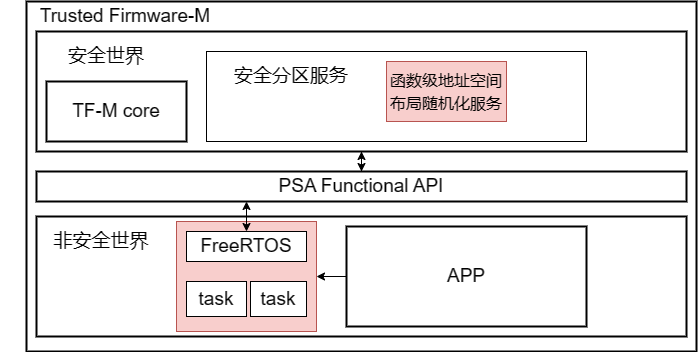
\includegraphics[scale=0.5]{graph/picture of all works.png}
    \caption{系统架构设计}
    \label{fig:system_architecture}
\end{figure}
\par 如图\ref{fig:system_architecture}所示,本项目系统架构设计如下:

\begin{itemize}
    \item \textbf{TrustedFirmware-M(TF-M)框架}:利用TrustedFirmware-M,我们可以为设备的安全性提供一个可靠的基础。这个开源框架提供了一种用于保护设备的方法,包括安全启动,固件更新和安全服务。它也提供了与安全性相关的各种API,让开发人员可以更容易地实现安全功能。
    \item \textbf{函数级地址空间布局随机化服务(ALSR)}:本项目中,我们将函数级地址空间布局随机化服务(ALSR)作为安全服务运行在设备的安全分区中,从而保证其安全性。ALSR服务的主要功能是对设备的固件进行函数级随机化加载,从而防御内存破坏攻击。
    \item \textbf{实时操作系统FreeRTOS}:FreeRTOS是一个小型的实时操作系统内核,我们在非安全世界中运行FreeRTOS并通过函数随机化的安全服务进行重新加载,从而实现对设备的实时调度和安全执行。
\end{itemize}

\subsection{系统实现方案}

\subsubsection{基于 TrustZone-M 的函数级动态随机化加载技术}
\paragraph{系统设计}
\subparagraph{系统架构}
\par 本项目的设计基于 TrustZone 的函数级地址空间布局随机化技术 fASLR(Function-based ASLR)。fASLR 的系统架构如下图所示,fASLR 由四个主要功能组成部分组成:(i)编译模块(Compile Module,CM),(ii)静态信息提取(Static Information Extraction,SIE),(iii)启动引擎(Boot Engine,BE),以及(iv)函数随机化引擎(Function Randomization Engine,FRE)。
\begin{figure}[h]
    \centering
    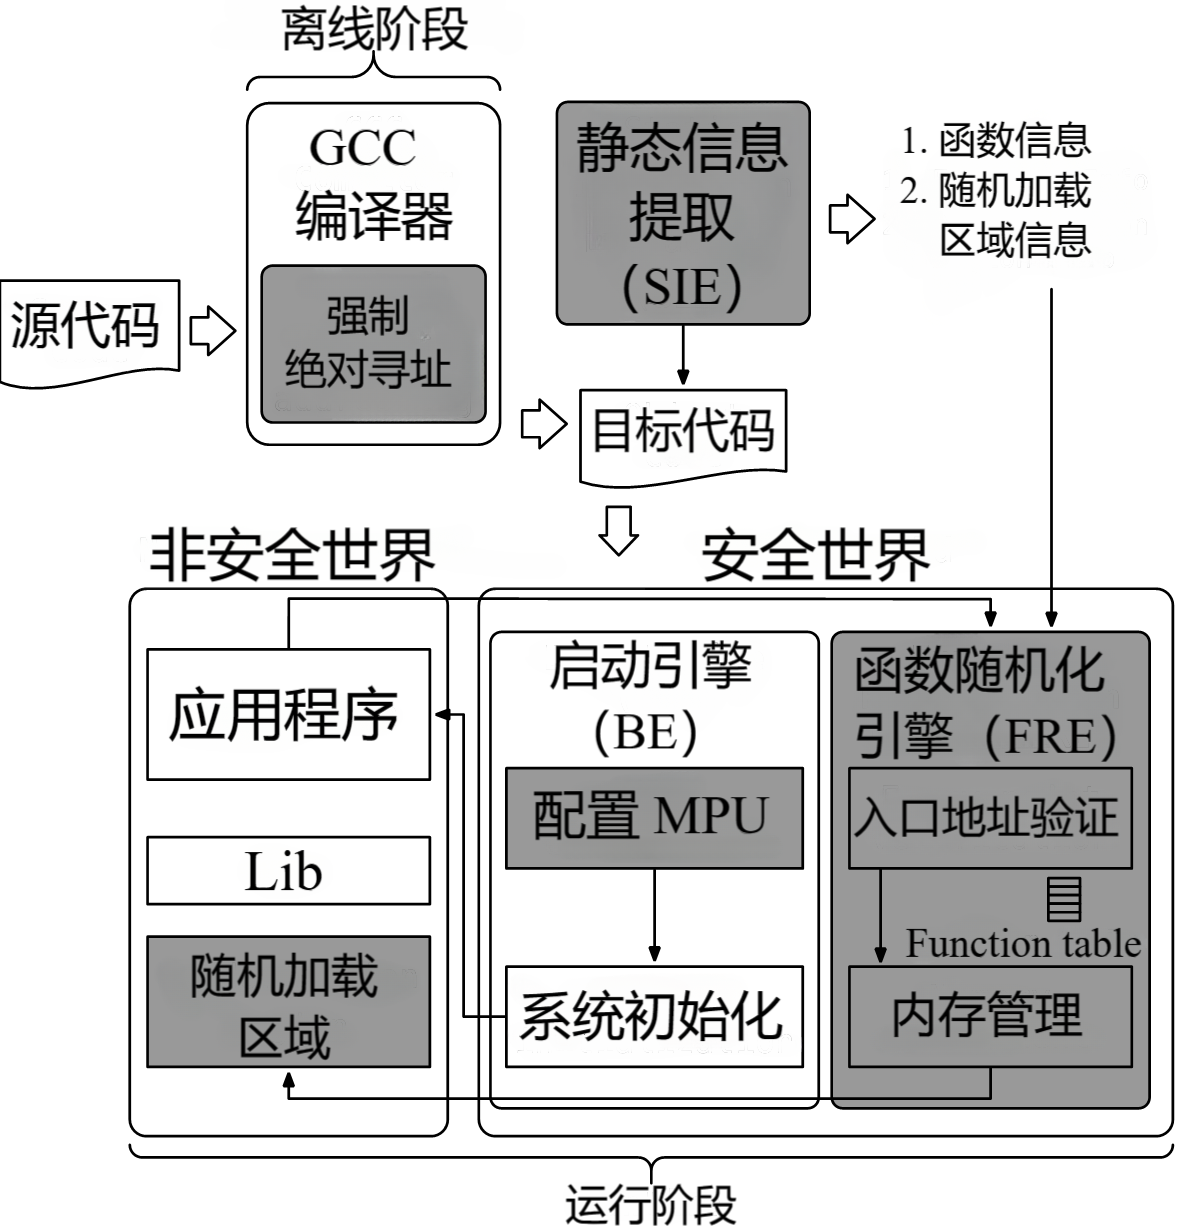
\includegraphics[scale=0.5]{graph/aslr_architecture.png}
    \caption{fASLR架构设计}
\end{figure}
\par 在离线阶段,fASLR 首先通过 CM 对应用程序进行编译,然后通过 SIE 对编译后的可执行文件进行信息提取,为之后系统运行时对函数进行随机化加载做前期准备。在系统运行阶段,BE 负责对系统进行配置以对应用程序代码进行保护,然后将控制权交给非安全世界的应用程序。最后,在应用程序的运行过程中,由 FRE 负责对其所有函数进行动态的随机化加载。
\par \textbf{编译模块(CM)}:编译模块的目的是使应用程序在函数间调用时采用绝对寻址模式。在 ARMv8-M 架构下,函数间调用可能存在两类寻址模式的跳转指令:绝对寻址模式和间接寻址模式。然而,由于 fASLR 的目标是对应用程序进行以函数为粒度的随机化,每个函数的函数体需要被加载至随机内存地址空间。因此,函数体内部基于相对地址寻址模式指令在随机化后将不再指向原有函数,虽然可以根据随机化信息对此类指令进行运行时重写,但如此做将需要巨大的离线静态分析工作并且严重影响系统性能。为解决上述问题,CM 通过对 GCC 编译器使用特殊的编译标志(-mlong-calls,-fno-jump-tables)对应用程序以及相关库代码进行编译,最终使编译后的可执行文件采用绝对寻址模式。
\par \textbf{静态信息提取(SIE)}:SIE 主要有两个功能:(i)生成 Function Table。当非安全世界代码通过 GCC 编译生成 ELF 格式的目标文件时,SIE 从 ELF 符号表中将所有函数的入口地址以及函数代码大小信息,并且从 .debug\_frame section 中提取函数对应栈帧的大小信息。将每一个函数的上述信息作为表项,全部被存储在称为 Function Table 的数据结构中。(ii)确定随机加载区域。SIE 根据非安全世界应用程序的 ELF 目标文件确定嵌入式设备上空闲 RAM 内存区域,该内存区域在应用程序正常运行时不会被使用。在系统运行阶段,该区域将被 FRE 用于随机化加载函数。
\par \textbf{启动引擎(BE)}:当支持 TrustZone-M 的设备启动时,启动流程按照先后顺序分别是安全世界 Bootloader,安全世界应用程序以及非安全世界应用程序。非安全世界应用程序首先启动 Reset Handler 作为其第一个函数执行。BE 作为安全世界 Bootloader 的一部分存储在安全世界的 Flash 内存。它负责配置内存保护单元(MPU)以使非安全世界代码在 Flash 上不可执行,这样做有两个目的:(i)MPU 保护非安全世界的应用程序以抵御代码复用攻击。(ii)当非安全世界在 Flash 上应用程序被设置为不可执行时,Flash 上任何代码执行会触发 MPU 硬件异常,该异常由安全世界的 HardFault Handler 进行异常处理。
\par \textbf{函数随机化引擎(FRE)}:FRE 作为 HardFault Handler 异常处理的一部分,负责函数的随机化加载,它的主要功能是将被调用的函数加载至随机加载区域并执行该函数。FRE 由函数入口地址验证(Function Entry Point Verification)模块以及内存管理(Memory Management)模块两部分组成。
\par 每当产生 HardFault 异常时,FRE 从异常栈帧中提取当前异常的返回地址(在正常情况下该返回地址为被调用函数的入口地址)。函数入口地址验证负责对该返回地址与 Function Table 中的函数入口地址进行匹配直到匹配成功。这样做有两方面原因,一方面该验证可以判断该异常是否是由正常函数调用所触发。因为有许多情况会引起 HardFault 异常,比如说,攻击者可以通过代码复用攻击执行一条不属于函数入口的指令。因此,该验证可以确保只有当函数入口指令触发异常时才会启动随机化机制。另一方面,通过对 Function Table 中函数入口地址的匹配可以获得该函数的代码大小以及函数栈帧信息,以便后续对其进行随机化加载。
\par 当 FRE 执行完函数入口地址验证后,内存管理模块负责为该被调用函数在随机加载区域随机的分配一块与函数体代码大小一致的 RAM 内存空间并对该函数进行加载(将该函数代码从 Flash 内存复制到已指定的 RAM 内存)。另外,若随机加载区域的 RAM 内存不足则会对已经完成执行的函数进行清理以保证每一次对函数的随机化有足够的内存空间供其被加载。随机加载区域的内存管理在内存受限的场景下具有一定难度,为此本项目设计了一种面向受限内存的函数级随机化内存管理机制并将在项目具体实现章节对其进行具体介绍。函数加载完成后,FRE 恢复该函数的上下文并使其在随机加载区域执行,在该过程中,本项目需要维护非安全应用程序的控制流以及其处理器模式以保证其正常运行。然而,函数随机化后,当前的控制流处于 HardFault 异常处理状态中,因此,本项目需要将控制流从异常处理状态转移至随机加载区域的被调用函数。尽管可以使用跳转指令直接从异常处理跳转至随机加载区域的函数入口,但该操作会破坏函数原有的调用栈从而导致函数的上下文不一致。另外,在 ARMv8-M 架构下,处理器在异常处理时总是处于 handler 模式,且其访问级别为特权态,因此直接使用跳转指令从异常处理机制恢复原来的处理器模式,可能使被调用函数的处理器模式前后不一致且存在越权的安全隐患。为解决上述问题,本项目对异常栈帧进行重写,修改其中的返回地址为被调用函数在随机加载区域的函数入口地址。至此,当异常处理机制执行返回操作时,硬件将异常栈帧中保存的上下文信息进行恢复,并且将异常栈帧中的异常返回地址(即被调用函数在随机加载区域的函数入口地址)赋于处理器的 PC 寄存器。因此在下一个处理器时钟周期处理器将返回至随机加载区域并重新执行被调用函数,同时,处理器模式也恢复为触发异常前的状态。

\subparagraph{工作流程}
\par 离线阶段:离现阶段主要负责代码编译以及烧录。在 GCC 编译器编译和链接非安全世界应用程序时,SIE 根据其 ELF 目标文件生成 Function Table。Function Table、BE 以及 FRE 被烧录至安全世界的 Flash 内存,而非安全世界应用程序的固件则被烧录至非安全世界的 Flash 内存。
\par 运行阶段:部署 fASLR 的系统运行时,所有对 Flash 内存上函数的调用都会将该函数加载至随机加载区域并执行。具体来说,当系统运行过程中一旦有产生函数调用,系统会跳转至被调用函数 callee 进行执行,由于 callee 对应的代码存储在 MPU 所保护的 Flash 内存上,因此系统尝试执行 callee 代码时将会触发 MPU 异常处理。此时,FRE 在 MPU 异常处理中对 callee 进行随机化加载,然后将控制流从 callee 在 Flash 内存的代码转移到该函数在随机加载区域的代码并恢复 callee 的执行。类似的,在 callee 的执行过程中,由于所有 callee 产生的函数调用依然指向 Flash 内存的函数代码,因此同样会触发 FRE 对其进行随机化加载至随机加载区域并执行。在函数执行完成后,函数将会返回至随机加载区域,并继续执行其被调用位置的下一条指令。FRE 通过上述方式对所有指向 Flash 内存的函数调用进行随机化并保证函数的正常执行。
\par 设备上电后,安全世界的 BE 对 MPU 进行相关配置然后启动非安全世界程序的 Reset Handler。Reset Handler 执行一系列的初始化操作后将会执行非安全世界的 main 函数,其中,Reset Handler 和 main 函数都会触发函数随机化加载,两个函数的函数体代码都会被 FRE 随机化加载至 RAM 内存中的随机加载区域中并执行。同样的,在 main 函数的执行过程中,一旦 main 函数中产生对 Flash 内存上函数的调用,控制流会被 FRE 所截获并对该函数进行随机化加载然后在随机加载区域恢复该函数的执行。以此类推,所有的函数都会被加载至随机随机加载区域执行。
\par 下图为程序在部署fASLR情况下的系统进行函数调用时的工作流程示意图,该图展示了函数X、Y、Z之间的调用过程,调用顺序为X调用Y,Y调用Z,图中$X^{'}、Y^{'}、Z^{'}$分别对应函数X、Y、Z在随机加载区域的函数体。该流程图包括运行过程中的函数调用(\ding{172}和\ding{175})、MPU异常处理(\ding{173}和\ding{176})、运行时函数随机化、函数执行(\ding{174}和\ding{177})以及函数返回(\ding{178}和\ding{179})。该流程图假设函数X已被加载进随机加载区域并从函数$X^{'}$开始执行,当$X^{'}$调用Y时(\ding{172})将会导致MPU异常(\ding{173})并触发HardFault Handler中的FRE。然后FRE将Y加载至随机加载区域并将控制流转移给$Y^{'}$(\ding{174})。在$Y^{'}$的执行过程中,$Y^{'}$将会调用Y,MPU异常再次被触发(\ding{175})并交给FRE进行处理(\ding{176}),控制流再次转移至$Z^{'}$。当$Z^{'}$执行完成后,控制流将会从$Z^{'}$返回至$Y^{'}$,再由返回至$X^{'}$。
\begin{figure}[h]
    \centering
    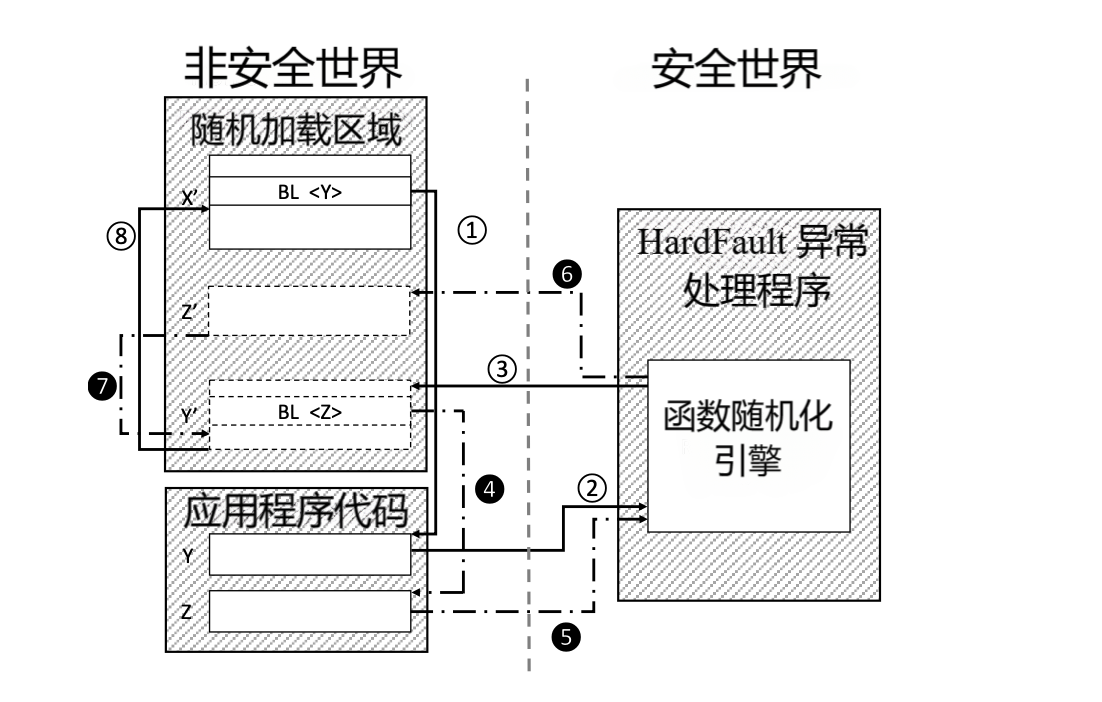
\includegraphics[scale=0.8]{graph/workflow.png}
    \caption{fASLR系统工作流程}
\end{figure}
\paragraph{面向受限内存的函数级随机化内存管理}
\par 与通用系统的内存管理一样,针对随机加载区域的内存管理不仅决定系统能否正常运行,而且对系统性能起着关键性影响。面向受限内存的函数级随机化内存管理的设计目标是在受限内存场景下,为能够随机化加载函数,实现高效的内存分配以及回收机制,保证系统可以正常运行并尽量不影响系统性能。
\par 通常来说,内存管理机制会对空闲内存进行地址连续的空间分配。但在需要对函数进行随机化加载的场景下,为保证分配内存的地址随机性,内存将会被切割成大小不一的不连续地址块,最终导致内存碎片化(Memory Fragmentation)。为实现对碎片化内存的高效管理,本论文设计了一种碎片化内存随机管理机制。
\par 尽管碎片化内存随机管理机制负责对内存进行回收,但如何选取回收内存的对象以及回收的时机至关重要。这一点决定了系统是否能够存在足够的内存以对函数进行随机化加载。具体来说,针对内存受限的深度嵌入式设备,在函数加载过程中可能会出现内存不足的情况,即其随机加载区域内存大小可能不足以加载整个非安全世界应用程序代码并执行。因此,需要对已加载的函数进行内存回收,以确保有足够的内存分配给当前函数。然而,由于函数与函数之间具有关联性,随意对已加载的函数进行内存回收将会影响程序正常执行。例如存在若干函数未完成执行,这些函数可能调用了其他函数且该被调用函数未返回,一旦将此类函数的内存进行回收,那么当其调用函数返回时,其返回地址则是无效地址,最终导致不可预测的结果。因此,在回收前需对已加载函数进行筛选,识别已完成的函数并对其进行回收。然而,由于fASLR在系统运行时无法动态获取函数返回信息,识别已完成函数具有一定难度。为此,本论文设计了一种基于调用栈帧展开的函数完成识别机制。
\par 另一方面,由于内存回收具有一定的性能开销,选择合适的时机对内存回收不仅能够保证有足够内存用于函数加载,而且能减少内存回收次数从而降低系统的性能开销。此外,由于深度嵌入式系统中存在大量循环,循环内的函数会被不断调用。然而,对于未被回收内存的函数,任何对该函数的重复调用依然会触发异常从而导致FRE的随机化加载,频繁的函数加载会严重影响系统性能。为此,本论文设计了一种基于函数级缓存的内存回收机制,通过函数级缓存以提高内存利用率并减少函数加载次数。为减少内存回收次数,实现在合适时机对函数内存进行回收;为减少函数的重复加载,实现对已加载函数调用机制的优化。
\subparagraph{碎片化内存随机管理}
\par 内存管理的关键是要将随机加载区域的已用内存和空闲内存的边界进行统一高效的管理。碎片化内存随机管理机制的基本思路是将内存以块链表进行管理,以内存块的形式为函数分配大小匹配的内存。具体地,本论文采用隐式空闲块链表(Implicit Free Lists)的方式对内存块进行管理。内存块的数据结构如图4 3(a)所示,主要包括元数据、负载数据以及填充数据:元数据由内存块的大小、以及指向下一个内存块的指针组成;负载数据用于对函数代码的加载;填充数据用于内存对齐。为方便叙述,本论文将已加载的函数所占有的内存块称为函数块,而其余的内存块则称为空闲块。本节从内存分配以及内存回收两方面对碎片化内存随机管理机制进行详细介绍。
\begin{figure}[h]
    \centering
    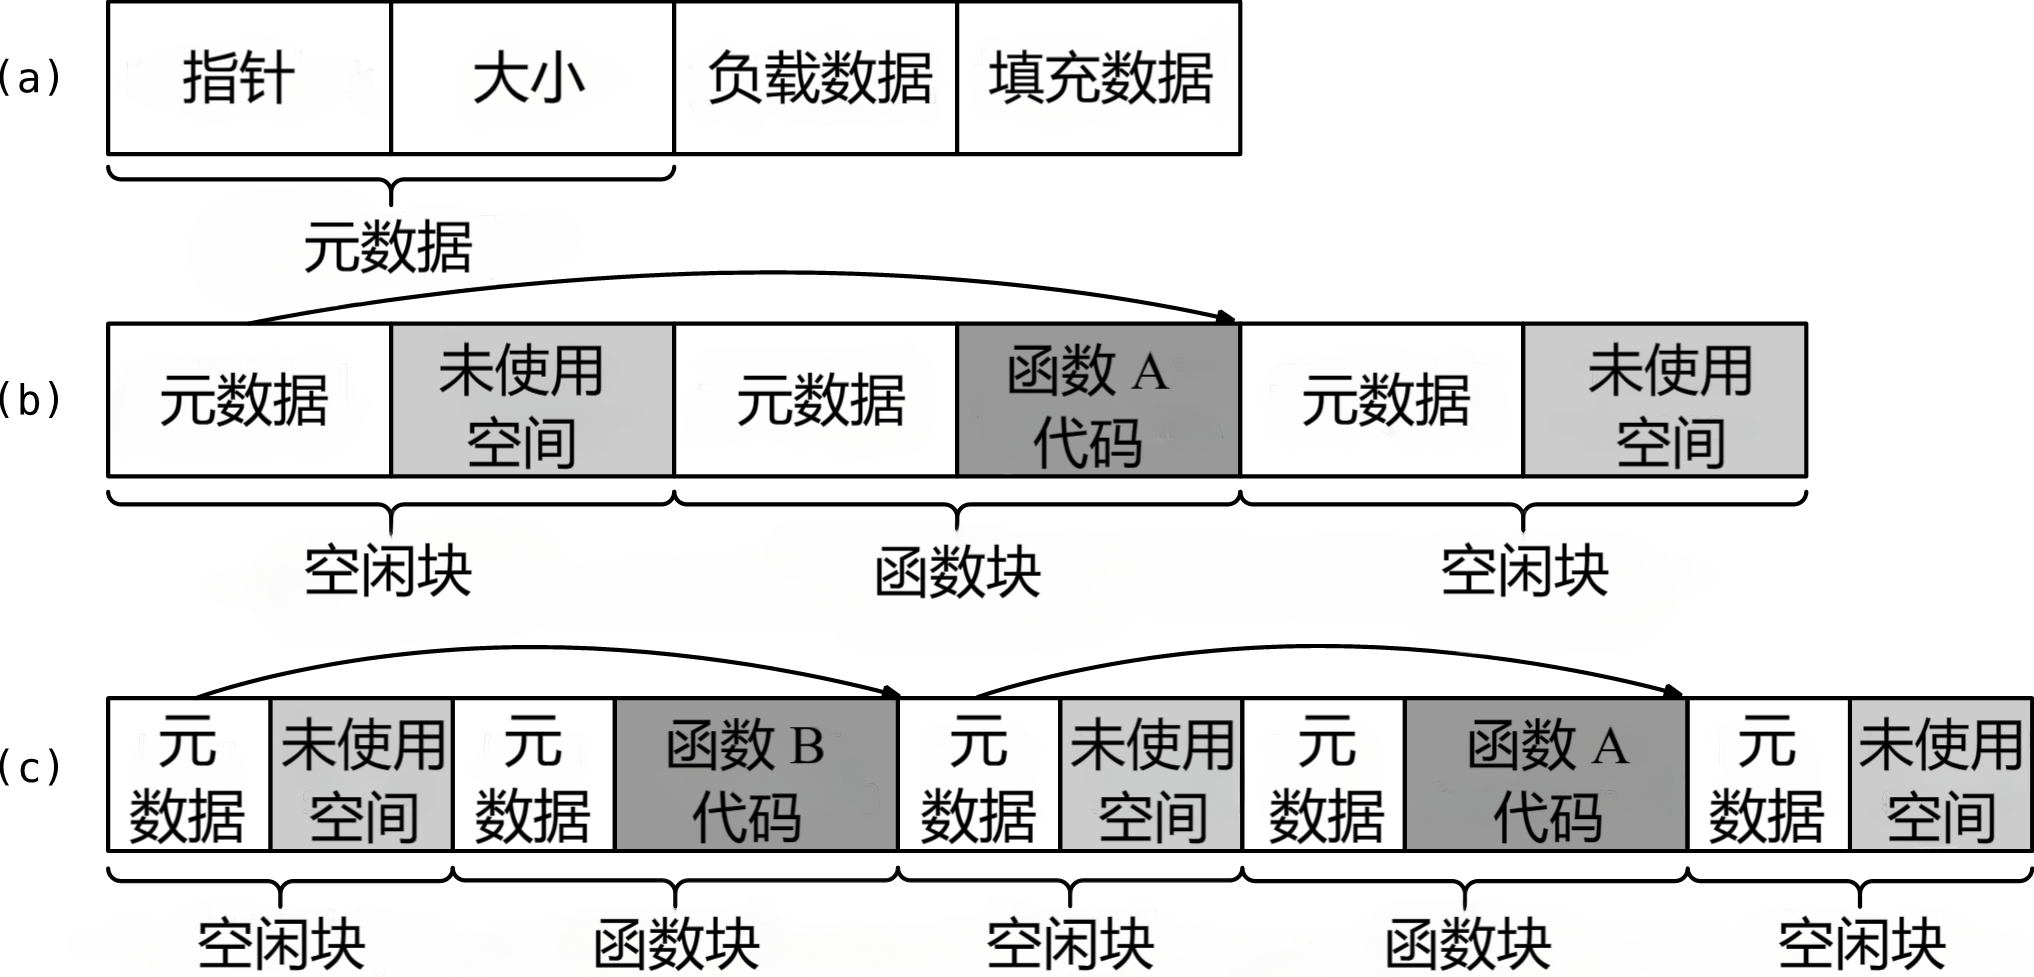
\includegraphics[scale=0.3]{graph/memoryManagement.png}
    \caption{基于隐式空闲链表的内存管理}
\end{figure}
\par 当系统启动时,FRE首先将整个随机加载区域初始化成一整个空闲块,加载若干函数后,该空闲块会形成一个空闲块链表。具体来说,当有函数需要被加载时,其函数体大小为$S_f$​,FRE首先扫描空闲块链表直到找到符合该函数体大小的空闲块,该内存块大小$S_b$​满足:
\[
    S_b-S_{meta}≥S_f
\]
\par 其中,$S_{meta}$表示元数据的大小。获得内存块以后,FRE从中随机的选取一个空闲块。由于用于函数加载的内存可能只占空闲块内存的部分,为了更高效的利用其余内存,FRE通过判断该内存块是否可以分裂成三个块:一块函数块以及两块空闲块。符合该条件的内存块大小应当满足:
\[
    S_b-3*S_{meta}≥S_f
\]
\par 对于不满足该条件的空闲块,直接返回其负载数据段的起始地址作为内存分配的地址。对于符合该条件的空闲块,则从该空闲块的负载数据段再次随机选取内存地址用于函数加载,最终由公式(4-3)得到内存分配地址address。同时,FRE根据该地址构建一个函数块,并对其余空闲内存构建两个空闲块插入原空闲块链表。举例来说,图4 3(b)表示在FRE在加载函数B前随机加载区域内存的状态,在当前情况下,函数A已被加载,且与其相邻的存在两个空闲块。当FRE加载函数B后,如图4 3(c)所示,函数块A左侧的空闲块分裂成三个部分,包括一个存放函数B代码的函数块及其相邻的空闲块。
\[
    address=ranom\%(S_b-3*S_{meta}-S_f)
\]
\par 内存的回收过程是将函数块插入空闲块链表的过程。具体地,FRE根据函数块的地址位置,扫描空闲块链表直到找到其在空闲块链表中对应插入位置。在插入过程中,FRE先判断该函数块是否能与其前一个空闲块或者后一个空闲块合并,最终合成新的空闲块链表。
\subparagraph{基于调用栈帧展开的函数完成识别}
\par 基于调用栈帧展开的函数完成识别机制的目标在于从当前所有已加载的函数识别出已完成执行的函数。对于当前正在执行的函数来说,本论文将其直接调用者及其间接调用者称为祖先函数(Ancestor Function)。在系统运行过程中,当前正在执行函数的祖先函数通常在等待其调用函数的返回,因此,此类函数的内存空间不能回收。除了当前正在执行的函数及其祖先函数,随机加载区域内其他已加载的函数称为已完成函数(Finished Function)。为识别已完成函数,本论文的基本思路是对所有已加载函数进行记录,然后根据当前调用栈信息识别出当前执行函数的所有祖先函数,最后从已加载函数中过滤所有祖先函数从而得到全部已完成函数。
\begin{figure}[h]
    \centering
    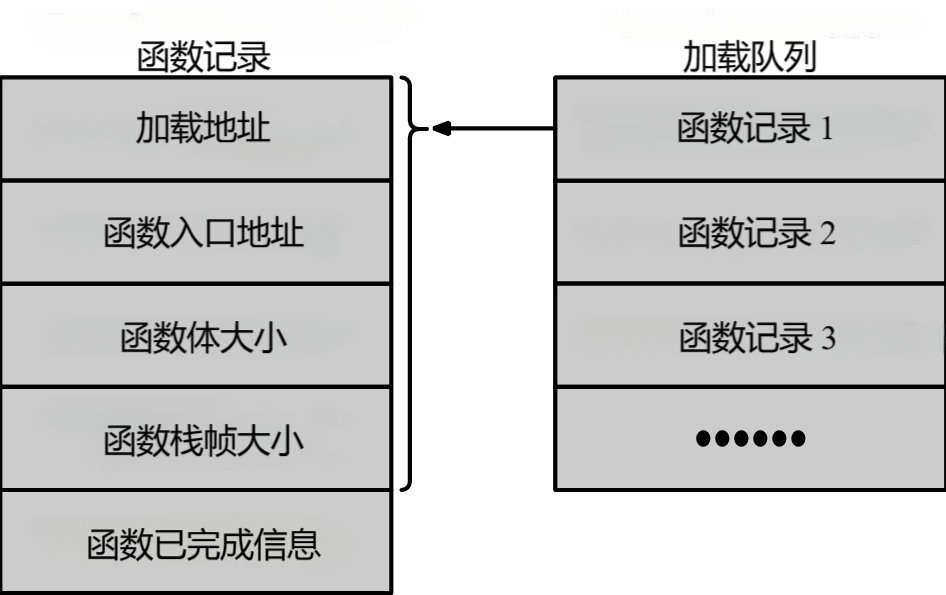
\includegraphics[scale=0.7]{graph/dataStructure.png}
    \caption{函数记录以及加载队列的数据结构}
\end{figure}
\par 具体地,FRE在每一次函数加载时会对该函数信息进行记录,用于表示函数信息的数据结构称为函数记录(Function Record)。如图4 4所示,一个函数记录包括:(i)该函数在随机加载区域的函数入口地址,(ii)该函数体的大小,(iii)函数栈帧大小,(iv)该函数已完成信息,(v)函数原始入口地址。其中,函数入口地址与函数体大小决定了该函数的加载区域范围,函数栈帧大小表示其在执行的时候所需要栈的大小,函数已完成信息表示该函数是否已完成执行,函数原始入口地址表示该函数在Flash内存中的入口地址。为对所有已加载函数进行记录,FRE用一个称为加载队列(Loading Queue)的数据结构以存储所有函数记录。
\par 调用栈通常被用于追踪函数执行流,在ARMv8-M架构中,一般情况下最先被压入函数栈帧的是函数的返回地址。因此,一旦确定了函数的栈帧,其栈帧最底部存放的值则是该函数的返回地址,从而根据函数记录的加载区域与该返回地址进行匹配以最终确定该函数的调用函数。FRE根据调用栈中存放的函数返回地址,在加载队列的函数记录中不断回溯其调用函数直到找到所有祖先函数,并对这些祖先函数对应的函数记录进行标记。
\begin{figure}[h]
    \centering
    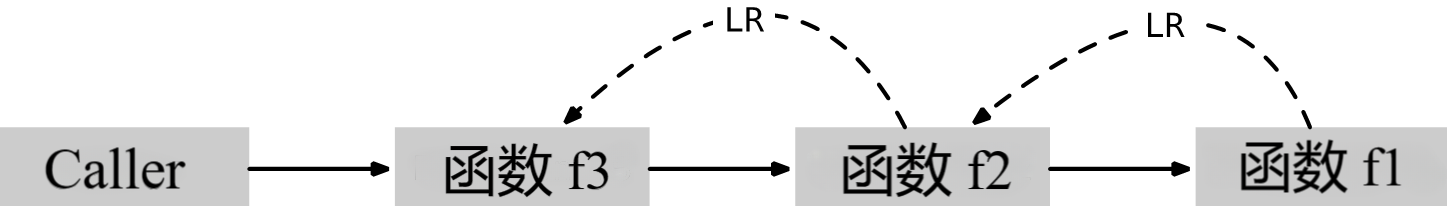
\includegraphics[scale=0.5]{graph/funcCall.png}
    \caption{f3、f2以及f1的函数调用关系}
\end{figure}
\par 具体而言,在如图4 5所示的调用过程中,其调用栈帧图如图4 6所示,当函数$f_0$被调用从而触发HardFault异常处理时,硬件自动将产生异常前的上下文信息通过异常栈帧保存,异常栈帧有固定大小$s_e$。FRE通过读取非安全世界的栈指针寄存器获得当前应用程序的栈指针SP并通过异常栈帧获得当前函数的返回地址$R_0$。此时,由于当前函数未被执行,栈上的第一个函数栈帧属于当前函数的调用函数$f_1$,其栈帧顶部地址$T_1=SP+s_e$。为获取$f_1$的调用函数,则需要获取其栈帧大小从而得到其函数返回地址,因此FRE需要定位$f_1$对应的函数记录。它对加载队列中的函数记录进行扫描直到$R_0$恰在某一函数记录对应的加载区域内,则该函数记录所对应的函数即为$f_1$。然后,FRE根据$f_1$的栈帧大小$s_1$可以确定$f_1$的调用函数$f_2$的栈帧顶部地址$T_2=T_1+s_1$。由于$f_1$的返回地址存放在其栈帧底部,即与$f_2$栈帧顶部$T_2$相邻,因此通过$T_2$可以得到$f_1$的返回地址$R_1$。同样的,根据$R_1$和$T_2$可以从加载队列中得到$f_2$的函数记录、$T_3$以及$f_2$的返回地址$R_2$。重复上述过程,FRE可以根据调用栈帧展开得到当前函数的所有祖先函数$f_1、f_2、f_3……f_n$,并在加载队列中对其函数记录标记为已完成。
\subparagraph{基于函数级缓存的内存回收}
\par 基于函数级缓存的内存回收机制的目标是提高随机加载区域内存利用率以优化系统性能。其基本思路是尽可能的将已加载函数放置在随机加载区域,将其作为FRE函数加载时的函数级“缓存”。
\begin{figure}[h]
    \centering
    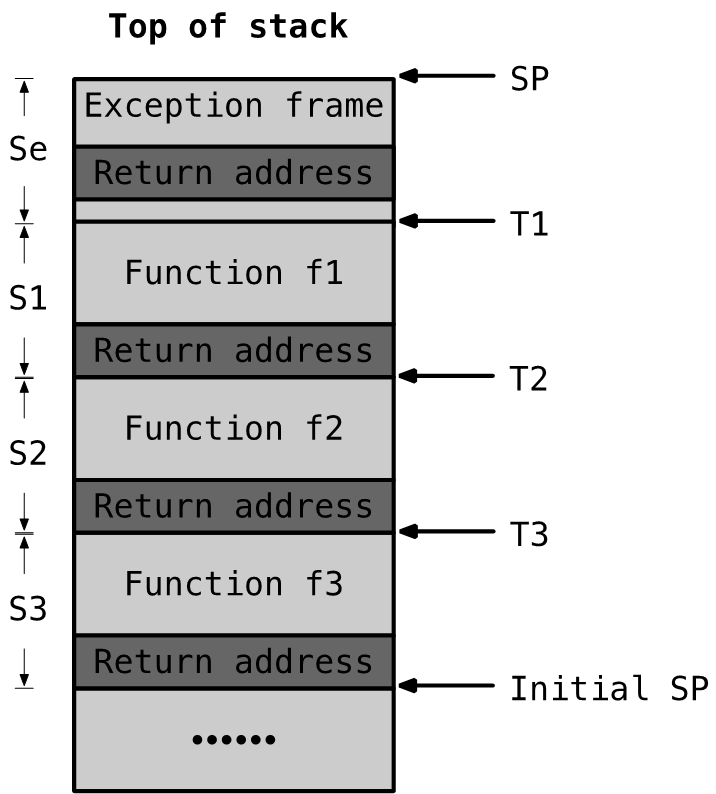
\includegraphics[scale=0.7]{graph/stackFrame.png}
    \caption{函数调用栈帧结构}
\end{figure}
\par 具体地,FRE使用函数记录保存已加载函数信息,并将其放入加载队列,该加载队列即为函数缓存。当FRE对当前函数进行加载时,它首先通过异常栈帧获得函数的原始入口地址,随后通过该地址与加载队列中的函数记录进行匹配,从而判断该函数是否已存在缓存中。若是,则称为函数缓存命中(Function Cache Hit),此情况下FRE不再对该函数进行随机化加载,而是直接根据函数记录得到该函数在随机加载区域的函数入口地址并恢复该函数的执行。若不是,则称为函数缓存缺失(Function Cache Miss),此情况下FRE按照原执行流程对该函数进行随机化加载。在函数级缓存基础上,为进一步减少函数加载次数,提升系统性能,本论文设计了函数调用重定向以及函数内存按需清理。
\par 函数调用重定向:函数调用重定向是通过优化重复函数调用以减少重复的函数加载。其基本思路是针对当前已被加载的函数,对其被调用点(即该函数的调用函数调用该函数的指令所在位置)对应的函数入口地址值进行重写,使该函数调用所指向的函数入口地址由该函数在Flash上的对应地址变为在随机加载区域的对应地址。具体地,当函数调用触发FRE的随机加载机制时,FRE会判断该函数是否已在函数缓存中,若是,则说明该函数目前正在被重复加载。因此,FRE通过异常栈帧找到该函数的返回地址,并由此找到该函数的被调用点并对该调用点对应的函数入口地址值进行重写使其指向该函数在随机加载区域的函数入口地址。至此,下一次对该函数的调用则会直接跳转至随机加载区域而不触发FRE。举例来说,如图4 7所示,在系统运行过程中函数A将会重复调用函数B,函数B在随机加载区域的加载地址为0x20002c00,在未进行函数调用重定向时,函数A每次对函数B的调用都将会触发MPU异常并经由FRE对其进行加载并执行。在启用函数调用重定向的fASLR情况下,在函数A第二次调用函数B时,FRE根据函数的函数入口地址查找发现函数B的函数记录已存在函数缓存中,随后FRE根据异常栈帧中LR寄存器的值以获得函数A调用函数B的指令位置,即blx指令的下一个指令所在的地址,FRE对该blx指令的机器码进行解码得到其跳转寄存器为R3,然后FRE向上遍历寻找对R3的赋值指令(图4 7中的movw以及movt指令)并对其进行重新编码以将其跳转地址改为函数B在随机加载区域的加载地址,修改完成后,函数A对函数B的调用将会被直接重定向至随机加载区域而不再触发MPU异常,从而大大减少了异常触发的频率,极大减少了其所带来的性能开销。
\begin{figure}[h]
    \centering
    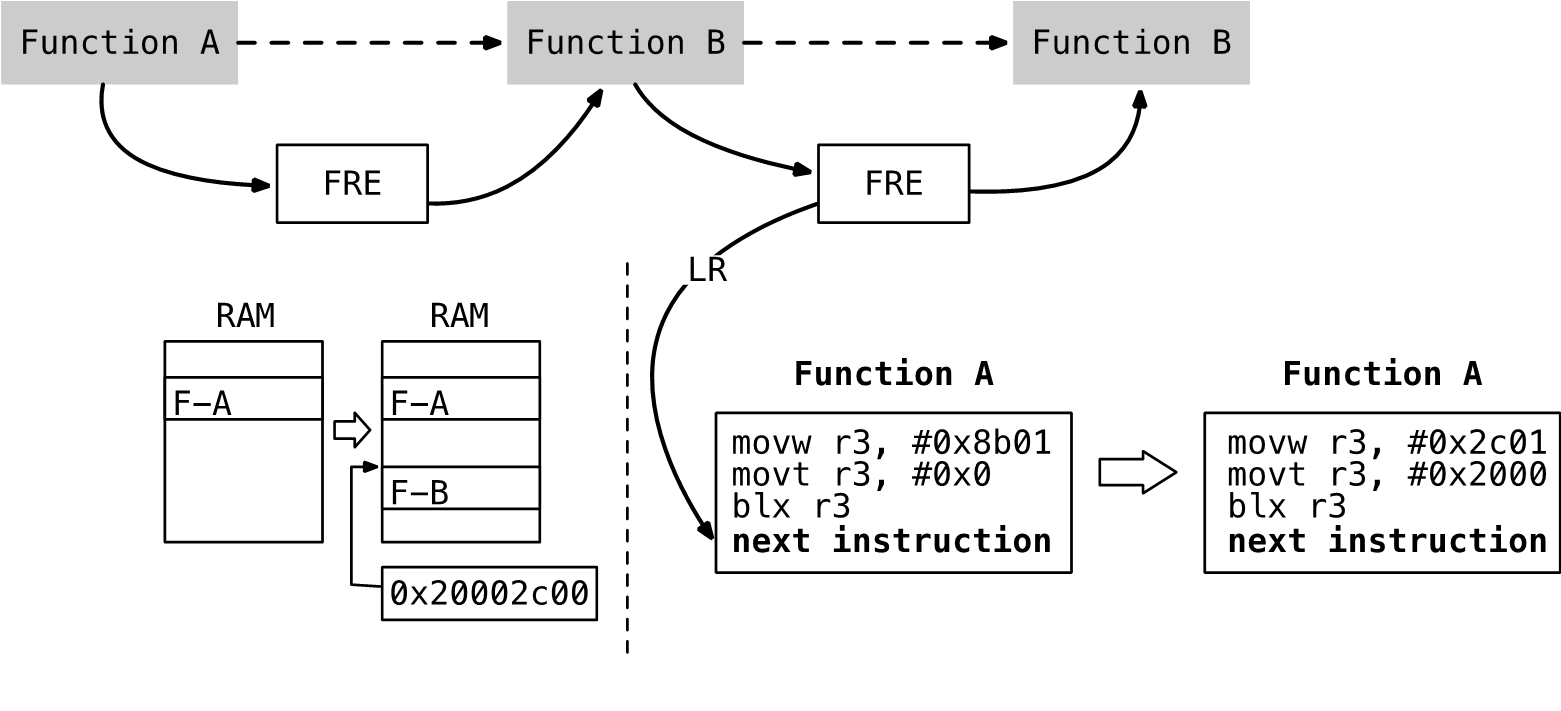
\includegraphics[scale=0.5]{graph/redirection.png}
    \caption{函数调用重定向}
\end{figure}
\par 此外,由于FRE可能随时对某个函数内存进行回收,对该函数的被调用点进行重写则会使下一次调用该函数时跳转至无效的函数入口,从而导致意想不到的后果。因此,FRE构建一个重写链表(Rewriting List)用于统一保存所有重写的信息(重写的位置及其原值),并在函数内存回收前根据该重写链表对重写过的调用点进行还原。
\par 函数内存按需清理:函数内存按需清理是为保证在有足够内存用于函数随机化加载的情况下尽可能减少内存回收的次数,通过提高函数缓存利用率以减少函数加载次数。FRE仅在当前随机加载区域内存不足以加载当前函数时才会执行内存回收。在对函数进行随机化加载前,FRE首先检查是否有足够内存加载该函数。若没有,FRE会根据重写链表还原被重写的调用点,然后利用基于栈的函数完成识别机制在函数缓存(即加载队列)中对所有已完成函数进行标记,最后将函数缓存中所有标记的函数执行内存回收并更新函数缓存。


\paragraph{自动化脚本ELF-To-FUNCS}
\subparagraph{ELF-To-FUNCS的简介}
\par 为提高工程效率,减少人工出错的可能性,我们编写了自动化脚本ELF-To-FUNCS。本脚本利用Python以及第三方库pyelftools对elf文件进行解析,并且对相应的函数信息进行提取。同时,利用提取的信息修改Function table。
\par 由于本脚本基于跨平台编程语言Python,因此不受不同操作系统和不同环境的约束,部署简单,可移植性高。
\subparagraph{ELF-To-FUNCS的实现}
\par ELF (Executable and Linking Format)指可执行和可链接格式,最初是由UNIX系统实验室(USL)开发和发布的,作为应用程序二进制接口(ABI)的一部分。现在Linux、FreeBSD、macOS等许多操作系统中都有广泛的应用。参照TIS协会制定的elf标准文档1.2版本,可知elf文件主要由图\ref{elf}所示的几个部分构成。其中,在Sections中存在.symtab节和.debug节。在.symtab节中包含符号表(Symbol Table),在debug节中保存有关符号调试的信息。
\begin{figure}
    \centering
    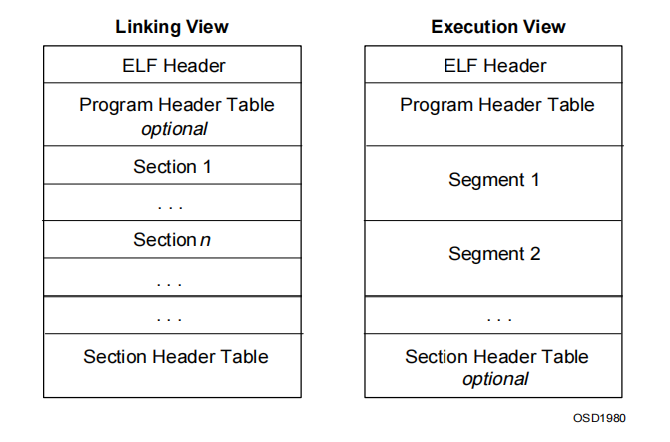
\includegraphics[scale=1.2]{graph/elf_struct.png}
    \caption{ELF结构图}
    \label{elf}
\end{figure}
\par 如图\ref{sf},在符号表中包含了STT\_FUNC符号,该符号与一个函数或其他可执行代码相关联。
\begin{figure}
    \centering
    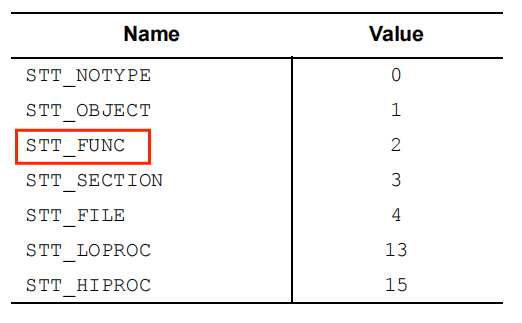
\includegraphics[scale=1.2]{graph/stt_func.png}
    \caption{符号表部分结构图}
    \label{sf}
\end{figure}
\par 并且基于符号表的结构:
\begin{verbatim}
    typedef struct { 
Elf32_Word st_name; 
Elf32_Addr st_value; 
Elf32_Word st_size; 
unsigned char st_info; 
unsigned char st_other; 
Elf32_Half st_shndx; 
} Elf32_Sym;
\end{verbatim}
\par 我们就可以通过提取elf的符号表中的STT\_FUNC符号来获取函数信息,然而,对于不同的操作系统,其对elf解析的实现有所不同,因此我们采用跨平台编程语言Python作为脚本的开发工具,具体的,我们利用pyelftools中的dwarfinfo模块,获取sections中的符号表,定位到STT\_FUNC符号,找到对应的函数信息,进行提取保存。
\par 同时,如图\ref{df}所示在本系统的elf文件中存在.debug\_frame节,debug\_frame是一种调试信息,它是用于支持栈回溯的一种数据结构。在程序崩溃或者出现异常时,栈回溯是一种快速诊断和解决问题的方法。由于程序在运行时会使用堆栈来保存临时变量和函数调用信息,因此栈回溯需要了解每个被调用函数的参数、返回地址和局部变量等信息。这些信息都保存在debug\_frame中。debug\_frame通常由两个部分组成:FDEs(Frame Description Entries)和CIEs(Common Information Entries)。CIEs包含了所有与堆栈回溯相关的通用信息,比如访问寄存器的方式、数据类型、偏移量等等。一个CIE可以对应多个FDE。FDEs包含了与具体函数相关的信息,如该函数在代码段中的起始和结束地址、stack frame layout等,它们可以通过CIEs进行索引查找。如果找到了函数对应的FDES就可以获取其起始地址,对Function table进行修改。
\begin{figure}
    \centering
    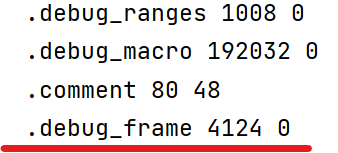
\includegraphics[scale=1]{graph/debug_frame.png}
    \caption{.debug节内容}
    \label{df}
\end{figure}
\par 具体的,我们利用pyelftools中的callframe模块,提取CIE和FDE信息,如图\ref{id}的‘initial\_location’即为函数首地址。
\begin{figure}
    \centering
    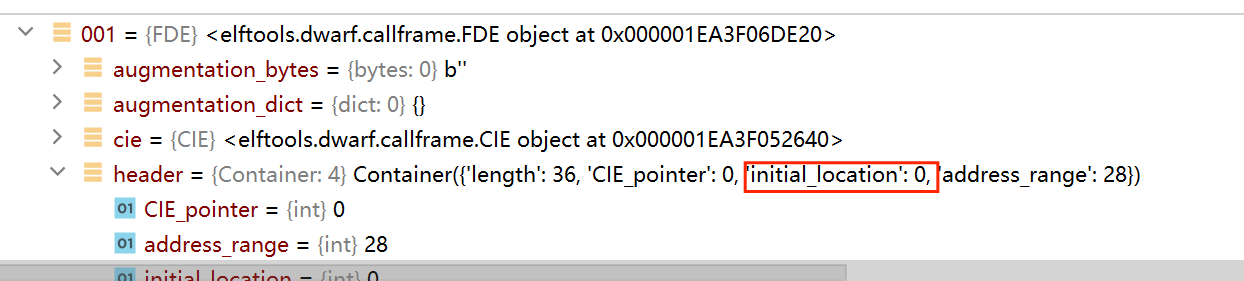
\includegraphics[scale=0.3]{graph/initial_addresspng.png}
    \caption{FDE对应首地址}
    \label{id}
\end{figure}
\par 通过上述工作,我们最终将脚本整合成以下结构:
\begin{itemize}
    \item config.ini:配置文件,包含重要文件的路径。
    \item ELF\_frames\_sizes.txt:用于保存提取出的函数地址以及调用帧大小信息。
    \item funcs.txt:用于保存从elf文件中提取出的函数信息。
    \item funcs\_sizes.txt:用于保存包含调用帧大小的函数信息。
    \item funcs.c: 样例文件,本文件为函数列表的样例。
    \item frame\_parser.py: 框架解析文件,本文件用于解析elf文件,获取相应信息。
    \item main.py: 本文件用于修改`func.c`文件。
    \item tutorial.md: 本脚本的使用教程。
\end{itemize}
\par 在使用前只需要填写config.ini的elf文件的路径<Elfpath>和需要修改的函数表的路径<func.c Path>即可,实现对函数信息的自动化修改。



\subparagraph{ELF-To-FUNCS的优势}
\begin{itemize}
    \item 自动化操作:本脚本可以自动地完成函数表的修改,从而减少了人工操作。在传统的手动修改中,需要对每个函数表项进行逐一修改,容易出现疏漏或者错误。而本脚本可以自动化地完成这个过程,减少了出错的可能性,同时也提高了开发效率。
    \item 精确性高:本脚本利用 ELF 文件格式规范来定位和操作函数表,避免了手动修改过程中可能出现的错误。手动修改时,可能会误操作或者定位不准确,从而影响程序的正确性和稳定性。本脚本利用了文件格式规范,能够精确地定位和操作函数表,从而保证了修改的准确性和稳定性。
    \item 良好的可移植性:本脚本使用跨平台编程语言Python作为开发工具,并利用其提供的第三方库pyelftools。在不同系统或者环境下都能够良好地运行,不需要对代码进行大量修改或者适配。这使得部署变得更加简单,并且提高了代码的可移植性和灵活性。
    \item 可扩展性好:本脚本采用了良好的软件工程实践,可以根据需要进行修改和定制,以满足不同应用场景下的需求。脚本中的代码结构清晰,函数模块化,易于阅读和维护。这意味着可以在需要的情况下轻松地扩展新的功能或者修改现有的功能,从而使脚本更加适合不同的使用情境。
\end{itemize}


\subparagraph{ELF-To-FUNCS的应用场景}
\par ELF-To-FUNCS主要应用于软件开发和维护领域,除了本系统中用于嵌入式开发,自动修改其函数信息。使用本脚本还可以定位到需要修改的函数表,并修改其中相应函数的指针。除此之外,在软件升级过程中,需要更新旧版本中的某些函数。使用本脚本可以方便地解析 ELF 文件,定位到函数表所在的段,并修改其中的函数指针,实现函数替换操作。并且在软件逆向工程或者漏洞挖掘过程中,需要对 ELF 文件进行修改以绕过某些安全检测或者实现某些攻击。使用本脚本可以快速定位到需要修改的函数表,插入指定的函数指针,从而达到相应的目的。
综上,本脚本可以广泛应用于软件开发和维护领域,能够为开发人员提供便利,降低出错的可能性,并且增强了软件开发和维护的效率。
\subparagraph{ELF-To-FUNCS的实例}
\par 现给出具体实例展示本脚本的使用流程及其可行性。
\begin{enumerate}
    \item 填充配置文件。
    \begin{enumerate}
        \item 如图\ref{gl},将待解析的elf文件路径填入<Elfpath>,本例改为\begin{verbatim}C:\Users\Robin\Desktop\GPIO_IOToggle_TrustZone_NonSecure.elf\end{verbatim},将需要修改的函数表路径写入<func.c path>,本例为\begin{verbatim}C:\Users\Robin\Desktop\funcs.c\end{verbatim}
        \begin{figure}
            \centering
            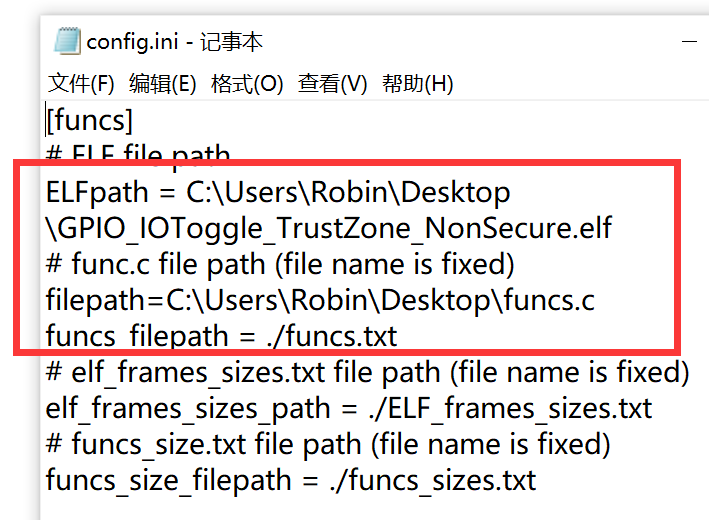
\includegraphics[scale=0.4]{graph/gailujing.png}
            \caption{填充路径}
            \label{gl}
        \end{figure}
        \item 如图\ref{xgq1}和图\ref{xgq2},依据函数表可知修改前`func.c`共有162个函数,并且部分地址尚未改变。
        \begin{figure}
            \centering
            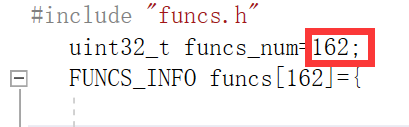
\includegraphics[scale=1]{graph/xiugaiqian1.png}
            \caption{func.c修改前1}
            \label{xgq1}
        \end{figure}
        \begin{figure}
            \centering
            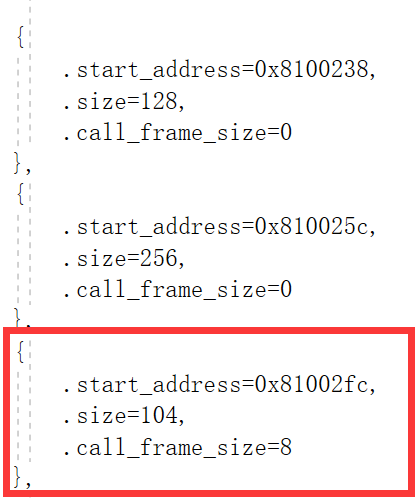
\includegraphics[scale=0.5]{graph/xiugaiqian2.png}
            \caption{func.c修改前2}
            \label{xgq2}
        \end{figure}
      \end{enumerate}
    \item 终端运行脚本
    \begin{enumerate}
      \item 运行结果如图\ref{yx}:
      \begin{figure}
        \centering
        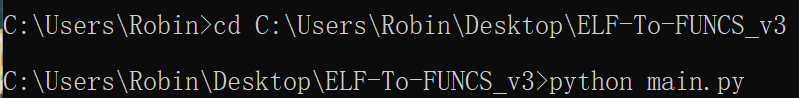
\includegraphics[scale=0.5]{graph/zhongduanjieguo.png}
        \caption{运行结果}
        \label{yx}
    \end{figure}
      \item 输出函数信息以及解析数据如图\ref{sc}:
      \begin{figure}
        \centering
        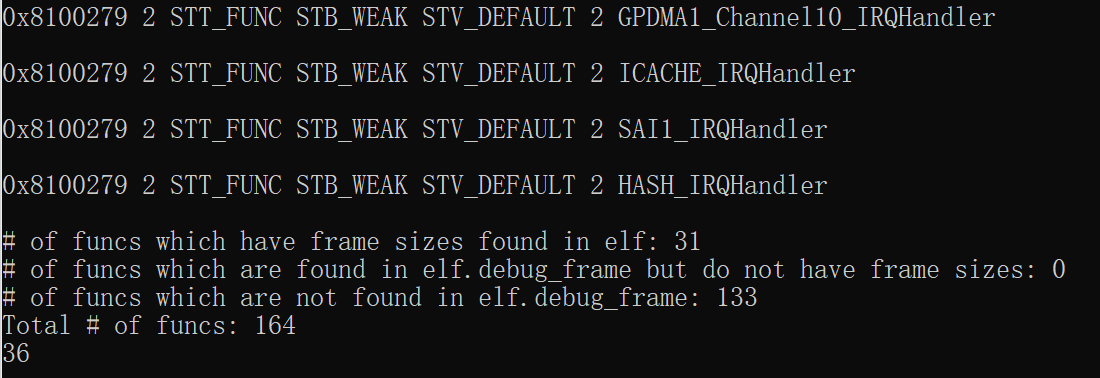
\includegraphics[scale=0.3]{graph/shuchujieguo.png}
        \caption{输出函数信息以及解析数据}
        \label{sc}
    \end{figure}
      \item 如图\ref{xg1},func.c被成功修改:
      \begin{figure}
        \centering
        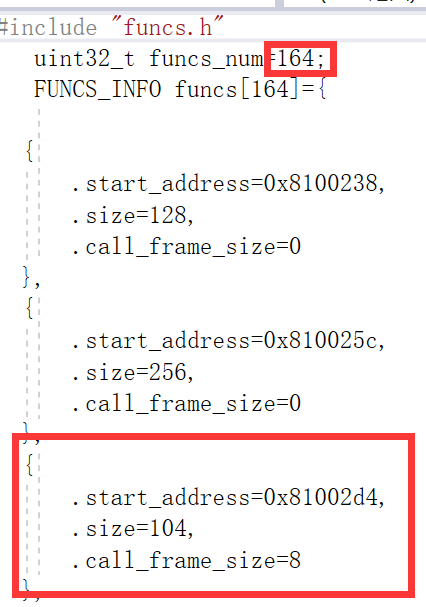
\includegraphics[scale=0.5]{graph/xiugaihou.png}
        \caption{func.c修改后}
        \label{xg1}
    \end{figure}
    
      
    \end{enumerate}
  \end{enumerate}
\par 依据上例可见,本脚本成功修改函数表,具有可行性。


\subsubsection{Trusted firmware-M系统架构}
\paragraph{TF-M简介及设计目的}
\subparagraph{TF-M简介}
\par Trusted Firmware-M(TF-M)是由Arm开发的开源固件项目,旨在为物联网(loT)设备提供安全的运行环境。TF-M旨在提供一个可配置和可裁剪的安全固件平台,以支持从小型嵌入式设备到高端安全系统的多种应用场景。TF-M的架构是模块化的,允许使用者在不影响其他模块的情况下添加或删除安全服务。
\par TF-M 采用了两个核心概念:Secure Processing Environment(SPE)和Non-Secure Processing Environment(NSPE)。SPE 是一个安全执行环境,可以保护关键数据和代码免受未经授权的访问和修改。NSPE 是一个普通的执行环境,可以访问所有的硬件资源。TF-M 提供了一组安全服务,例如安全启动、加密解密、密钥管理、认证和授权等,这些服务可以在SPE中运行,以保证安全性。
\subparagraph{TF-M设计目标}
\par TF-M的设计目标是保护互联网设备上的敏感数据和代码免受攻击,它需要满足以下需求:
\begin{itemize}
    \item 安全性:TF-M 旨在为 IoT 设备提供安全的运行环境,以保护设备和用户数据免受攻击。
    \item 可配置性:TF-M 的架构是模块化的,允许用户根据自己的需求配置和定制安全服务。
    \item 易于集成:TF-M 提供了一个标准接口,使得其他软件可以轻松地与TF-M 集成。
    \item 可移植性:TF-M 可以在不同的硬件平台上运行,并且支持多种处理器体系结构。
    \item 易于维护:TF-M 的代码是模块化的,易于理解和维护。
\end{itemize}

\paragraph{TF-M系统设计}
\subparagraph{TF-M架构设计}
\par TF-M的系统整体架构设计如下图所示。整个TF-M部署在安全世界(SPE)中,为安全/非安全世界提供安全服务,主要由安全启动(Secure Boot)、TF-M内核(TF-M Core)以及安全服务(Secure Service)组成。
\begin{figure}
    \centering
    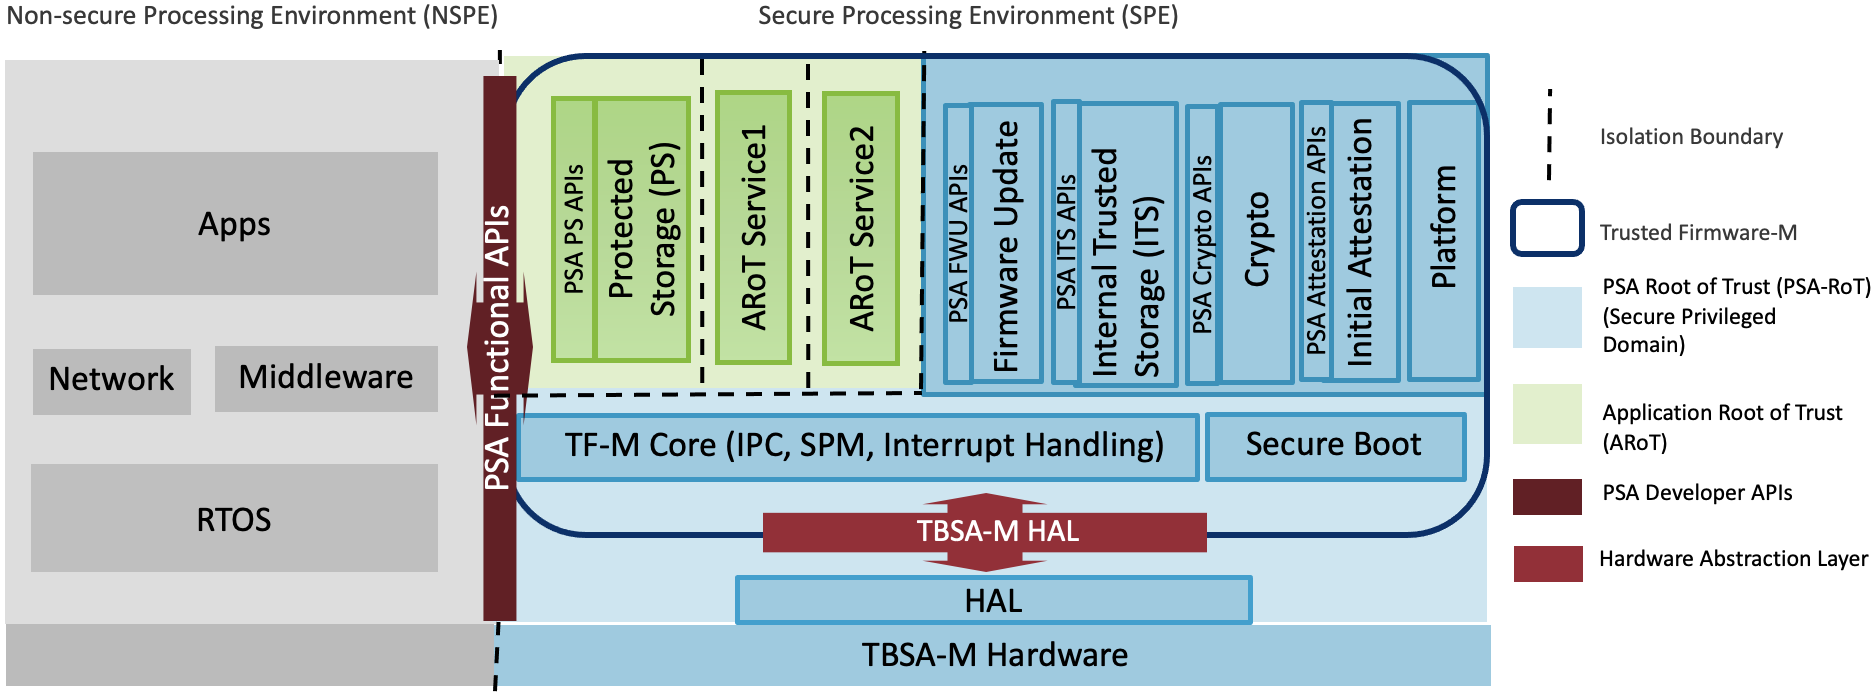
\includegraphics[scale=0.2]{graph/readme_tfm_v8.png}
    \caption{Trusted Firmware-M架构图}
\end{figure}
\par 在Trusted Firmware-M的背景下,安全启动负责在固件映像被加载和执行之前验证其真实性和完整性。它通过根据设备安全引导固件中存储的一组受信任的密钥检查固件映像的数字签名来执行此验证。安全启动可以对SPE (Secure Processing Environment)和 NSPE (Non-Secure Processing Environment)固件映像进行身份验证。NSPE映像在设备的非安全世界中执行,而SPE映像在安全世界中执行。如果固件映像未通过Secure Boot验证,则会被拒绝,设备将无法执行它。这可以防止攻击者在设备上执行未经授权的代码,从而保护设备及其数据免受恶意活动的侵害。
\par TF-M内核是TF-M的主要组成部分之一,它是一个基于微内核的安全操作系统内核。TF-M core的主要功能是提供安全隔离、通信控制和安全执行,主要模块包括IPC、SPM、Interrupt Handling。其中,IPC 用于在SPE和 NSPE之间进行通信。它提供了一种安全的方式,以便在受保护的环境内传递数据和控制信息。SPM用于管理和控制在SPE中运行的各个安全分区。SPM使得多个安全分区可以在同一硬件平台上运行,并且可以互相隔离。Interrupt Handling用于管理和处理来自设备的中断请求。TF-M内核通过在SPE和NSPE之间传递中断请求,确保了所有中断的安全处理。TF-M内核还包括一些其他的辅助模块,比如Secure Entry/Exit和Secure Attribution等,用于在SPE和NSPE之间进行安全的上下文切换和资源分配。
\par 安全服务负责向安全/非安全世界提供具有较高安全需求的功能实现并由安全内核负责对其进行调用,如安全储存、安全启动、加密等。每一个安全服务具有唯一标识符SID(Service ID)且有统一的函数调用入口。为统一调用接口,每个安全服务都可以通过SID和version两个参数被非安全世界用户进行调用,其中,SID参数是要调用的安全服务的唯一标识符,version是请求的信任根服务版本。NSPE的用户通过PSA API发送请求后,由SPM将请求打包成消息并转发到相应服务处理程序的函数。
\par TF-M拥有特定的隔离机制,以保护一个保护域的信息免受从其他域访问,故TF-M中不同区域间的访问需要特定的PSA API来实现,后续将详细解释TF-M的通信机制。

\subparagraph{TF-M隔离机制}
\par PSA针对不同设备的安全性、性能、成本提出了三个级别的隔离,如下图所示。第一级隔离将SPE与NSPE隔离开,NSPE不能访问SPE的资源,需要由PSA client API访问特定的服务。第二级隔离在第一级隔离的基础上,引入了PSA RoT和Application RoT隔离边界。这两类服务不能访问各自的资源,需要由PSA API访问对方的服务。第三级隔离在前两级的基础上引入了对每个安全分区之间的隔离边界,实现对所有安全分区的隔离,其是最高级别的隔离。
\begin{figure}
    \centering
    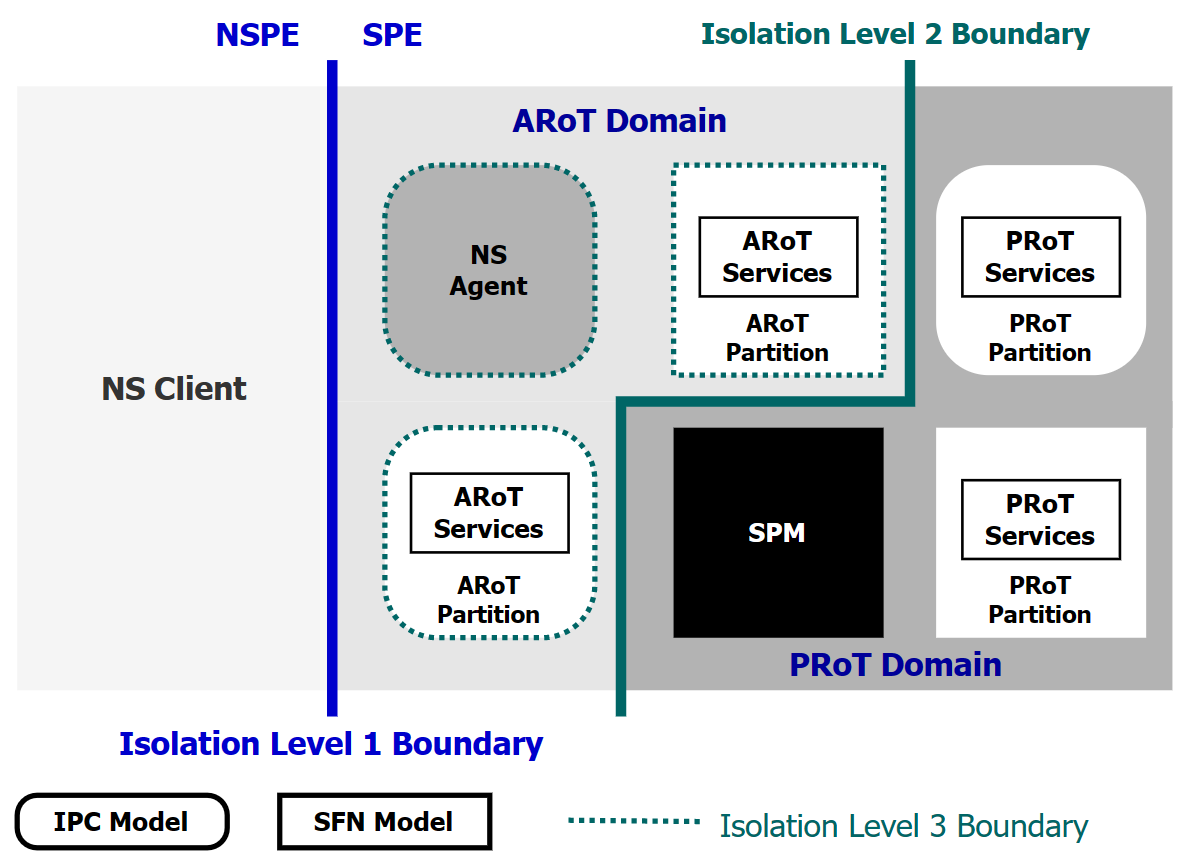
\includegraphics[scale=0.27]{graph/isolation.png}
    \caption{TF-M隔离机制}
\end{figure}
\subparagraph{TF-M提供的安全服务}
\par Trusted firmware-m提供了一系列安全服务来保护设备和应用程序的安全,以下简要介绍一些TF-M提供的安全服务:
\begin{itemize}
    \item 安全更新(Secure Firmware Update):提供了对设备固件的安全更新和回滚功能,以确保固件的完整性和真实性。
    \item 安全存储(Secure Storage):提供了一个安全的存储区域,用于保存设备的机密信息,例如密钥和证书。
    \item 安全连接(Secure Connection):提供了一些加密和认证技术,用于建立安全的设备到设备(Device-to-Device)或设备到云(Device-to-Cloud)连接。
    \item 安全运行时环境(Secure Runtime Environment):提供了一个隔离的安全环境,在这个环境中执行的代码和数据与其他非安全代码和数据隔离开来。
    \item 安全调试(Secure Debug):提供了一些安全的调试技术,以便开发人员在不破坏设备安全性的情况下对设备进行调试和测试。
    \item 安全网络协议(Secure Network Protocols):提供了一些安全的网络协议,例如TLS和DTLS,用于保护设备与其他设备或云服务之间的通信安全。
    \item 安全固件(Secure Firmware):提供了一些安全的固件实现,例如安全的虚拟化技术,以确保设备的安全性。
    \item 安全证书管理(Secure Certificate Management):提供了一些安全的证书管理技术,以确保设备的证书的安全性和完整性。
    \item  安全启动(Secure Boot):用于验证启动代码的完整性和真实性,确保只有受信任的代码被执行。
\end{itemize}
这些安全服务可以根据设备的需求进行配置和组合,以实现设备的安全性和可信度。

\subparagraph{安全分区运行机制——SFN模式与IPC模式}\par TF-M 实现了 PSA-FF-M 定义的IPC和SFN机制,以允许隔离固件分区之间的通信。IPC model和SFN model的主要区别如下:
\begin{itemize}
    \item IPC(Inter-Process Communication)模型是一种进程间通信模型,它允许不同的进程之间相互通信和协作,从而共同完成任务。TF-M中的IPC Model使用的是基于消息队列(Message Queue)的方式进行通信。每个安全服务都有一个消息队列,其他安全服务可以向该队列发送消息,通过消息队列,安全服务可以实现相互通信和协作。TF-M提供的安全启动、安全调试、安全存储等安全服务均采用IPC模式。
    \item SFN(Secure Function Call)模型是一种基于函数调用的安全模型,它允许不同的安全服务之间进行直接的函数调用。在TF-M中,安全服务被封装为一系列的安全函数,这些函数可以被其他安全服务直接调用,从而完成相应的安全操作。为了确保安全性,每个安全函数都被封装在一个受保护的安全域中,只有在该安全域中的安全服务才能调用该函数。TF-M提供的初始证明服务、加密、固件更新等安全服务均采用SFN模式。
\end{itemize}
IPC模式和SFN模式都是用于不同安全服务之间的通信和协作模式,IPC模式使用消息队列进行通信,更加灵活和可扩展,但安全性较差。SFN模式使用函数调用进行通信,安全性较好,但不太灵活。用户在自行编写添加安全服务时,具体选择哪种模型取决于应用场景的需求和安全性要求。

\subparagraph{TF-M架构中的各类API}
\par Trusted Firmware-M(TF-M)架构中包含了一系列的API,用于实现安全功能和提供安全服务。以下是TF-M架构中一些重要的API及其功能的详细介绍:
\begin{itemize}
    \item SST(Secure Storage Service)API:提供了对安全存储的访问和管理。SST API允许应用程序安全地读取、写入和删除存储在安全存储区域中的数据。
    \item ITS(Initial Trusted Service)API:用于设备的安全启动过程。ITS API提供了验证引导程序完整性、加载和执行可信固件的功能。它确保只有经过验证的固件能够在安全环境中启动。
    \item PSA(Platform Security Architecture)API:提供了一组通用的安全服务接口,用于实现设备的安全功能。PSA API包括加密、身份验证、安全认证、随机数生成等功能,可供应用程序使用。
    \item RoT(Root of Trust)API:用于建立设备的根信任,提供安全隔离和保护关键功能和数据的能力。RoT API用于创建和管理安全分区,确保关键代码和数据只能在受信任的环境中执行和访问。
    \item IPC(Inter-Processor Communication)API:用于在安全世界和非安全世界之间进行受控的通信。IPC API定义了安全接口,允许安全世界与非安全世界之间进行安全的数据传输和交互。
    \item Secure Partition Manager(SPM)API:用于管理和控制安全分区的运行。SPM API允许安全分区之间的隔离,并管理它们之间的资源分配和通信。
    \item Secure Gateway API:提供了对安全网关功能的访问,用于安全地与外部环境进行通信。Secure Gateway API允许安全世界与外部设备或网络进行加密通信和安全数据交换。
    \item Secure Debug API:用于在安全模式下进行调试和故障排除。Secure Debug API提供了安全的调试接口,允许对安全世界进行调试操作,同时保护关键数据的机密性和完整性。
\end{itemize}
\par 以上是TF-M架构中的一些重要API,它们提供了安全功能和服务的接口,用于实现物联网设备的安全性和可信度。通过使用这些API,开发者可以构建安全的应用程序和服务,保护设备免受各种安全威胁。

\subparagraph{TF-M源码文件夹结构分析}
\par 在TF-M的源码库中,有许多子文件夹,包括:
\begin{itemize}
    \item bl1:包含用于生成TF-M的第一级引导程序(BL1)的代码。此文件夹中的代码用于初始化系统环境并引导BL2。
    \item bl2:用于生成TF-M的第二级引导程序(BL2)的代码。此文件夹中的代码用于生成TF-M的第二级引导程序(BL2),该程序用于引导TF-M并配置系统环境。
    \item secure\_fw:包含实现安全功能的代码,如安全监控器和安全服务。此文件夹中的代码是实现TF-M核心安全功能的代码,包括安全状态机、安全中断处理、安全事件处理等。
          \begin{itemize}
              \item include:包含了一些必要的头文件,这些头文件定义了在    TF-M中需要使用的函数和变量等。
              \item partitions:用于将TF-M固件划分为不同的分区,每个分区都拥有自己的内存和安全级别。在这个文件夹中,开发者可以定义各个分区的大小和访问权限等。
              \item shared:包含了一些可供不同分区共享的资源,比如共享内存区域,共享的全局变量等。这些共享的资源在不同分区之间进行数据传输时需要进行安全性的保护。
              \item spm:安全分区管理器(Security Partition Manager)的缩写,是TF-M中一个重要的组件。spm文件夹中包含了spm的代码和配置文件,spm负责在不同的分区之间进行数据传输和安全性控制,以确保系统的安全性和可靠性。
          \end{itemize}
    \item interface:该文件夹包含与TF-M外部接口相关的代码,如TF-M API和外部接口函数。此文件夹中的代码是与外部系统的接口代码,包括TF-M提供的API函数、设备驱动程序接口、系统调用接口等。
          \begin{itemize}
              \item include:包含了一系列的头文件,这些头文件是开发者在使用TF-M时需要包含的文件,其中定义了TF-M的API接口、数据类型、错误码等信息,开发者可以使用这些头文件来编写TF-M的客户端代码,调用TF-M的API接口实现安全功能。
              \item src:开发者在使用TF-M时需要引用的文件,其中实现了TF-M的API接口,开发者可以使用这些源文件来实现TF-M的服务端代码,提供安全功能服务。
          \end{itemize}
    \item lib:用于实现基本安全功���的库代码,如加密算法和哈希函数。此文件夹中的代码是用于支持安全服务的基本库函数,如随机数生成、哈希计算、加密解密算法等。
    \item tools:包含用于开发和调试TF-M的实用工具和脚本。例如,此文件夹中包含了与TF-M相关的调试脚本、测试脚本以及用于生成密钥和证书的工具等。
    \item platform:包含与平台相关的代码,如设备启动代码和外设驱动程序。此文件夹中的代码是为了支持不同的硬件平台,使TF-M能够运行在不同的处理器架构和芯片上。
    \item docs:TF-M的文档,如用户手册和开发人员指南。此文件夹中的文件包括各种文档、说明、手册等,用于指导开发人员使用TF-M进行开发。
    \item cmake:用于生成TF-M构建系统的CMake文件。此文件夹中的文件用于支持TF-M的自动化构建,包括CMake脚本和Makefile文件。
    \item config:用于配置TF-M的各种选项的配置文件。此文件夹中的文件用于配置TF-M的不同选项,如安全级别、存储器布局、加密算法、硬件平台等。
\end{itemize}

\subsubsection{安全/非安全世界安全通信机制}
非安全世界在调用安全世界的安全服务时,其整个通信过程如下图所示,可以分为三个阶段:(1)请求阶段:非安全世界任务发起安全服务的请求至特定的API并最终交给TF-M内核;(2)执行阶段:TF-M内核验证客户端的身份和权限,然后根据请求中指定的安全服务标识符,将请求转发给对应的安全服务并等待其响应结果;(3)响应阶段:安全服务执行结束并返回执行结果给 TF-M内核,TF-M内核收到安全服务的执行结果后,会根据请求的类型和参数,将结果通过特定API返回给客户端。
\begin{figure}
    \centering
    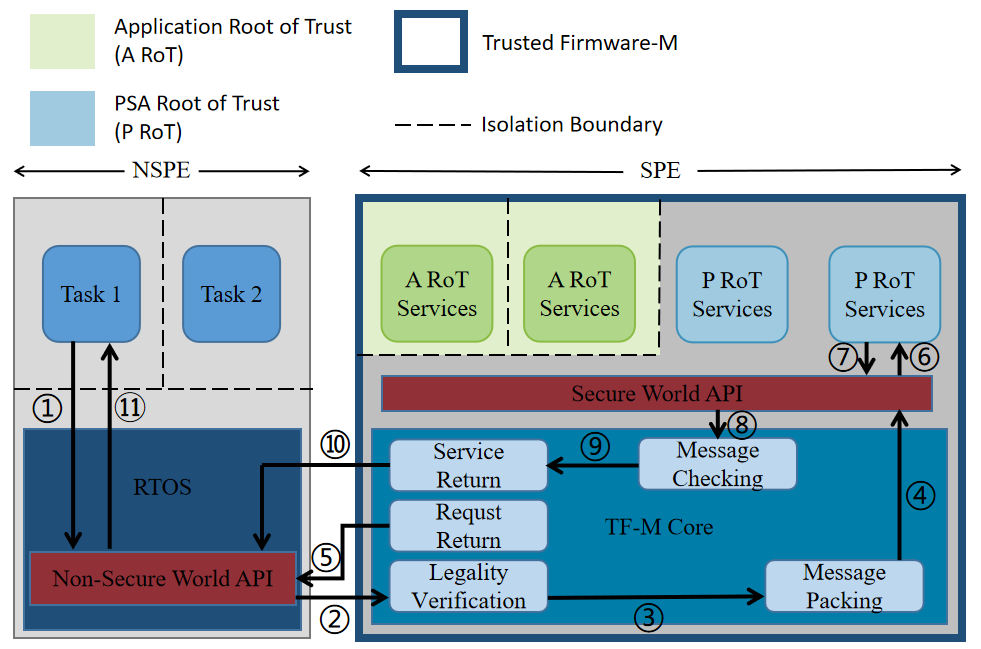
\includegraphics[scale=0.27]{graph/TF-M Secure communication processes.png}
    \caption{TF-M调用机制}
\end{figure}

\paragraph{请求阶段}
\par 客户端首先向 TF-M 提供的API接口发送请求。这些API接口包括tfm\_spm\_request(), tfm\_ns\_interface\_dispatch(), tfm\_secure\_api\_call()等。客户端发送的请求中包含要调用的安全服务的标识符,以及传递给安全服务的参数等信息,这些参数信息可以包括数据结构、指针等。之后,TF-M内核会接收客户端发送的请求,并在请求合法性验证通过后,根据请求中指定的服务标识符,选择相应的安全服务进行调用。在完成安全服务调用后,TF-M 内核会向客户端返回相应的结果,其中可能包括表示安全服务调用状态的状态码、加解密���的数据、安全服务抛出的异常或中断等。客户端可以通过 API 接口获取 TF-M内核返回的结果信息。
\par 上述过程中,TF-M内核在接收到API调用请求后,为防止有攻击者通过构造参数等方式对安全服务进行恶意调用,利用安全服务以访问安全世界的重要数据,会首先检查客户端的请求是否合法,检查包括以下内容:
\begin{itemize}
    \item 验证请求的来源:TF-M core会验证请求的来源,确保请求来自于受信任的客户端。这个过程可以通过验证请求中包含的认证信息,例如数字签名、证书等方式来完成。
    \item 验证请求的完整性:TF-M内核会验证请求的完整性,以确保请求的内容没有被篡改或者修改。这个过程可以通过使用消息认证码(MAC)等机制来完成。
    \item  验证请求的合法性:TF-M内核会验证请求是否合法,即请求中包含的安全服务标识符和参数是否合法。这个过程可以通过检查请求中包含的参数和标识符是否符合安全策略和规则来完成。
    \item  验证请求的访问权限:TF-M内核会验证请求的访问权限,即请求的客户端是否具有调用该安全服务的权限。这个过程可以通过检查请求的客户端身份和权限等信息来完成。
    \item  验证请求的时序性:TF-M内核会验证请求的时序性,即请求是否按照正确的顺序到达。这个过程可以通过使用时间戳等机制来完成。
\end{itemize}
\par 通过对请求进行上述合法性验证,TF-M内核可以确保安全服务的调用是合法、可信和安全的,同时避免了可能导致安全漏洞和风险的请求。

\paragraph{执行阶段}
\par 合法性验证之后,TF-M内核将请求的参数和其他相关数据打包成一个消息。消息包括要调用的安全服务的标识符,以及传递给安全服务的参数等信息。在打包过程中,TF-M内核会将消息进行加密和签名,以确保消息的机密性和完整性。之后,TF-M内核使用安全的通信机制将消息发送到安全分区。这个机制会在TF-M内核和安全分区之间建立的安全通信通道,它可以使用一些安全协议,例如TLS、IPsec等来保护通信的机密性和完整性,同时确保通信的可靠性。这个过程可以使用一些底层硬件设施来实现,例如硬件加速模块、安全内核等。安全分区接收到请求消息后,会对其进行解包。解包过程中,安全分区会验证消息的完整性和机密性,并使用相应的密钥解密消息内容。如果消息的完整性和机密性验证失败,安全分区会拒绝执行请求,否则,安全分区会继续执行请求。
\par 之后,安全分区根据请求中包含的标识符调用相应的安全服务,并传递相应的参数。在执行安全服务期间,安全分区可能会访问安全世界内的受保护资源,例如受保护的存储器、设备等。安全分区会使用安全策略和机制来确保这些资源不会被非安全世界访问或破坏。
\paragraph{响应阶段}
\par 在安全服务执行完成后,安全分区将执行结果打包成一个响应消息。响应消息包括响应码、执行结果以及其他必要的信息。之后,安全分区使用安全通信机制将响应消息发送回TF-M内核。TF-M内核接收到安全的响应消息后,首先对其进行验证。验证包括检查消息的签名和校验和,以确保消息的完整性和真实性。如果消息验证失败,则TF-M内核会丢弃消息并返回错误码。
\par 如果消息验证成功,则TF-M内核将解包响应消息,获取其中的执行结果和其他相关信息。最后,TF-M内核将响应结果返回给客户端。客户端收到响应结果后,可以进行下一步操作。
\par 需要注意的是,TF-M内核在处理响应消息时,需要使用与请求消息相同的安全通信机制。这是因为安全通信机制是建立在会话级别的,如果使用不同的通信机制,��导致安全通信中断,从而使得通信变得不可靠。

\subsubsection{基于 STM32L562E-DK 的 FreeRTOS 实时操作系统部署}
\par 实时操作系统(RTOS)是一种能够以足够快的速度接受并处理外界事件或数据的操作系统。它的主要特点是能够在规定的时间范围内控制生产过程或快速响应处理系统,并协调管理所有实时任务的运行。FreeRTOS是一款轻量级的开源实时操作系统,具有较小的内存占用和快速的任务切换速度,适用于资源受限的嵌入式系统。并且FreeRTOS具备良好的可移植性,可以在多种处理器架构和开发环境中使用,支持多种编译器和开发工具链。总的来说,FreeRTOS是构建高效、可靠和实时响应的嵌入式系统的理想选择。

\begin{itemize}
    \item[(1)] 下载源码:FreeRTOS 是一款遵循 GPLv2+ 许可协议的开源免费实时操作系统。直接从 FreeRTOS 官网下载源码。下载完成后,在项目文件夹下创建一个名为 FreeRTOS 的文件夹。FreeRTOS 源码包括 .c 文件(FreeRTOS 源码文件)、include 文件夹(相关头文件)、portable 文件夹(与编译器相关的文件夹,在不同的编译器中使用不同的支持文件)以及 MemMang 文件夹(与内存管理相关的文件夹)。此外,还有一个名为 FreeRTOSConfig.h 的文件,它是 FreeRTOS 的配置文件。

    \item[(2)] 将源码中的 .c 文件、include 文件夹和 portable 文件夹拷贝至创建的 FreeRTOS 文件夹中。在 portable 文件夹中,只保留 GCC 文件夹和 MemMang 文件夹,然后只保留 GCC 文件夹中的 ARM\_CM33 文件夹,以及 MemMang 文件夹中的 heap4.c 文件。接下来,将 Demo 文件夹下对应开发板的 FreeRTOSConfig.h 文件拷贝至项目的 include 文件夹中。

    \item[(3)] 配置 FreeRTOSConfig.h 文件:
        \begin{itemize}
            \item[(a)] 将 configENABLE\_TRUSTZONE 设置为 1,以支持 TrustZone 模式。
            \item[(b)] 将 configENABLE\_MPU 设置为 1,以支持内存保护单元(MPU)。
            \item[(c)] 注释掉原有项目自带的一些中断处理函数,以使用 FreeRTOS 提供的中断处理函数,例如 SysTick\_Handler、SVC\_Handler 等。
        \end{itemize}
\end{itemize}
\subsubsection{基于qemu模拟器运行的TrustedFirmware-M及自定义的安全服务}
\paragraph{简介}
\subparagraph{QEMU简介}
\par qemu是一个开源的仿真器,可以模拟多种CPU架构,包括ARM,MIPS,x86等。在本项目中,为了研究TF-M的架构和安全服务,而不是局限于设备的复杂硬件,前期我们基于qemu模拟ARM Contex-M33内核以运行TrustedFirmware-M。
\subparagraph{调试工具GDB}
因为本项目是使用gcc-arm-none-eabi工具链编译的,所以我们使用gdb作为调试工具。qemu会在调试模式下,开启一个gdb server, 我们可以通过vscode ssh远程连接到虚拟机,并通过gdb监听本地gdb server,实现对qemu的调试。
\paragraph{自定义的安全分区}
\subparagraph{介绍}
安全服务是一种执行环境,为Root of Trust (RoT)服务提供以下功能:
\begin{itemize}
    \item 访问资源,保护其自身的代码和数据。
    \item 与系统中的其他组件进行交互的机制。
    \item 每个安全分区是执行的最小单元,并具有隔离功能。 TF-M支持添加自己的安全分区,本项目中我们添加了一个简单的安全分区,用于测试非安全区与安全区的通信。

\end{itemize}
\subparagraph{实现}
\par 代码组织结构
\begin{lstlisting}
example_partition
|-- CMakeLists.txt
|-- tfm_example_partition.c           //核心代码
|-- tfm_example_partition.yaml        //提供安全分区的配置信息
|-- tfm_example_partition_api.c         
|-- tfm_example_partition_api.h         
|-- tfm_example_partition_secure_api.c//安全分区的API实现

\end{lstlisting}
\par 关键代码如下:
\begin{lstlisting}[language=C]{tfm_example_partition.c}
for(int i=0;i<1;++i)
{
    psa_read(msg.handle, 0, &read_buf, msg.in_size[i]);
    LOG_INFFMT("[Example partition] Service called from client[%d]\r\n",msg.client_id);
    LOG_INFFMT("%s\r\n",read_buf);
            
    psa_crypto_init();
    psa_hash_operation_t ho=psa_hash_operation_init();
    psa_hash_setup(&ho,PSA_ALG_SHA_256);
            
    psa_status_t st = psa_hash_update(&ho,(const uint8_t *)&read_buf,msg.in_size[i]-1);
    int length=0;
    st = psa_hash_finish(&ho,write_buf,32,&length);
    if(st==PSA_SUCCESS)
    {
        LOG_INFFMT("Crypto service called successfully, sha256 for the string is:\r\n");
        for(int k=0;k<length;++k)
             LOG_INFFMT("%X",write_buf[k]);
    }
    LOG_INFFMT("\r\n");
	psa_write(msg.handle, 0, write_buf, length);
}
\end{lstlisting}
\par 基于IPC模型,安全分区可以通过$psa\_read()$函数从非安全区读取数据,然后调用$psa\_crypto\_init()$函数初始化加密服务,最后调用$psa\_hash\_finish()$函数对数据进行哈希计算,最后将计算结果通过$psa\_write()$函数写回非安全区。
\subsection{实验成果展示}
\section{作品测试与分析}
\subsection{测试方案}
\subsection{测试环境搭建}
\subsection{测试数据及分析}
\section{创新性说明}
\section{总结}
\clearpage
\pagestyle{refStyle}
\bibliographystyle{unsrt}
\bibliography{ref}
\end{document}